\documentclass[10pt,portrait, twocolumn]{article}
\usepackage{multicol}
\usepackage{calc}
\usepackage[portrait]{geometry}
\usepackage{amsmath,amsthm,amsfonts,amssymb}
\usepackage{times}
\usepackage{color,graphicx,overpic}
\graphicspath{ {images/} }
\usepackage{hyperref}
\usepackage{pgfplots}
\usepackage{esint}

\usepackage{bm}
\usepackage{tikz}
\usepackage{color}
\usepackage{relsize}
\usepackage{datetime}
\usepackage[utf8] {inputenc}
\usepackage[spanish, activeacute] {babel}
\usepackage{IEEEtrantools}
\usetikzlibrary{arrows}

\usepackage{listings}
\usepackage{framed}

%\tikzset{
%     block/.style={rectangle, draw, fill=red!40, text width=6em,
%                   text centered, rounded corners, minimum height=3em},
%     arrow/.style={-{Stealth[]}}
%     }
\usetikzlibrary{backgrounds,calc,positioning, arrows}

\usepackage{pdflscape}

%Evita errores con el paquete de español y escribir flechas entre tikz nodos
\tikzset{
every picture/.append style={
  execute at begin picture={\deactivatequoting},
  execute at end picture={\activatequoting}
  }
}

%\usepackage{draftwatermark}
%\SetWatermarkText{Javier de Martín}
%\SetWatermarkScale{0.8}

% This sets page margins to .5 inch if using letter paper, and to 1cm
% if using A4 paper. (This probably isn't strictly necessary.)
% If using another size paper, use default 1cm margins.
\geometry{top=.5cm,left=.5cm,right=.5cm,bottom=.5cm}
    
\pgfplotsset{
    dirac/.style={
        mark=triangle*,
        mark options={scale=2},
        ycomb,
        scatter,
        visualization depends on={y/abs(y)-1 \as \sign},
        scatter/@pre marker code/.code={\scope[rotate=90*\sign,yshift=-2pt]}
    }
}

\lstset{language=C, % Use Perl in this example
        frame=single, % Single frame around code
        basicstyle=\small\ttfamily, % Use small true type font
        keywordstyle=[1]\color{Blue}\bf, % Perl functions bold and blue
        keywordstyle=[2]\color{Purple}, % Perl function arguments purple
        keywordstyle=[3]\color{Blue}\underbar, % Custom functions underlined and blue
        identifierstyle=, % Nothing special about identifiers                                         
        commentstyle=\usefont{T1}{pcr}{m}{sl}\color{MyDarkGreen}\small, % Comments small dark green courier font
        stringstyle=\color{Purple}, % Strings are purple
        showstringspaces=false, % Don't put marks in string spaces
        tabsize=5, % 5 spaces per tab
        %
        % Put standard Perl functions not included in the default language here
        morekeywords={rand},
        %
        % Put Perl function parameters here
        morekeywords=[2]{on, off, interp},
        %
        % Put user defined functions here
        morekeywords=[3]{test},
       	%
        morecomment=[l][\color{Blue}]{...}, % Line continuation (...) like blue comment
        numbers=left, % Line numbers on left
        firstnumber=1, % Line numbers start with line 1
        numberstyle=\tiny\color{Blue}, % Line numbers are blue and small
        stepnumber=5 % Line numbers go in steps of 5
}

% Turn off header and footer
\pagestyle{empty}

% Redefine section commands to use less space
\makeatletter
\renewcommand{\section}{\@startsection{section}{1}{0mm}%
                                {-1ex plus -.5ex minus -.2ex}%
                                {0.5ex plus .2ex}%x
                                {\normalfont\large\bfseries}}
\renewcommand{\subsection}{\@startsection{subsection}{2}{0mm}%
                                {-1explus -.5ex minus -.2ex}%
                                {0.5ex plus .2ex}%
                                {\normalfont\normalsize\bfseries}}
\renewcommand{\subsubsection}{\@startsection{subsubsection}{3}{0mm}%
                                {-1ex plus -.5ex minus -.2ex}%
                                {1ex plus .2ex}%
                                {\normalfont\small\bfseries}}
\makeatother

\newcommand{\Lagr}{\mathcal{L}}

% Define BibTeX command
\def\BibTeX{{\rm B\kern-.05em{\sc i\kern-.025em b}\kern-.08em
    T\kern-.1667em\lower.7ex\hbox{E}\kern-.125emX}}

% Don't print section numbers
\setcounter{secnumdepth}{5}


\setlength{\parindent}{0pt}
\setlength{\parskip}{0pt plus 0.5ex}

%My Environments
\newtheorem{example}[section]{Example}
% ---------------------------------------------------------------

\begin{document}


\begin{framed}
	\begin{center}
    	\Large{\underline{ASI}} \\
	\large{Primera Parte: S.O.} \\
    	\scriptsize{3º Ingeniería de Telecomunicaciones | UPV/EHU}\\
     	Actualizado por última vez el \today \\
     	"\textsl{Under-promise and over-deliver}." \\
     	%\hspace{5 pt} \\
     	\small{\textbf{Javier de Martín -- 2016/17}}
	\end{center}
\end{framed}

%%%%%%%%%%%%%%%%%%%%%%%%%%%%%%%%%%%%%%%%%%%%%%%%%%%%%%%%%%%%%%%%%
% Tema 4



\section{Introducción}

\subsection{Introducción}


Los ordenadores están equipados con una capa de software llamada \textbf{sistema operativo}, su trabajo es proveer programas con una interfaz para manejar los componentes del ordenador de una forma más simple.\\

El \textbf{procesador} corre en dos \textbf{modos}:

	\begin{itemize}
	\item \textbf{Usuario}: Dispone un conjunto limitado de instrucciones.
	\item \textbf{Kernel o Supervisor}: Tiene acceso completo a todo el hardware y puede ejecutar cualquier instrucción que la máquina puede ejecutar. El Sistema Operativo es software que corre en modo kernel.
	\end{itemize}

\begin{figure}[h]
	\centering
     \begin{tikzpicture}[
block/.style={
draw,
fill=white,
rectangle, 
minimum width={width("Kernel o Supervisor")+2pt},
font=\small}]
		\node[](acc){Modos Procesador};
		\node[block](gyro){Usuario};
		\node[block,below=0.1cm of gyro](mag){Kernel o Supervisor};
	\end{tikzpicture}	
      \caption{Modos del procesador}
  \end{figure}



\begin{figure}[!ht]
	\center
	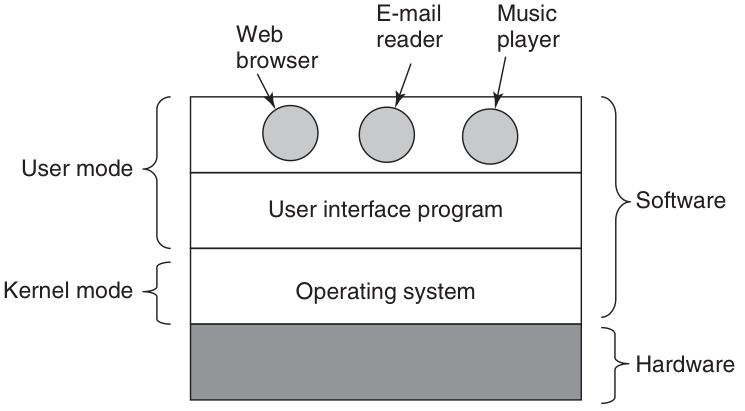
\includegraphics[width = .3\textwidth]{Estructura}
	\caption{Dónde encaja el sistema operativo}
\end{figure}

\subsubsection{Interface}

La \textbf{interfaz de usuario} es el nivel más bajo de software ejecutable en modo de usuario, permite al usuario arrancar otros programas.

\quad El sistema operativo corre sobre el hardware y provee la base para cualquier otro software que se ejecute.\\

Es importante distinguir entre el sistema operativo y software normal (modo de usuario). El usuario es libre de cambiar lo último pero no es posible modificar el sistema operativo.

\begin{figure}[h]
	\centering
     \begin{tikzpicture}[
block/.style={
draw,
fill=white,
rectangle, 
minimum width={width("Kernel o Supervisor")+2pt},
font=\small}]
%		\node[](acc){Modos Procesador};
		\node[block,below=0.1cm of acc](gyro){Usuario};
		\node[block,below=0.5cm of gyro](mag){Interfaz};
		\node[block,below=0.5cm of mag](mag2){HW};
		\node[left=0.5cm of mag](mag3){S.O.};
		\node[right=0.5cm of mag](mag4){(Máq. Extendida, Máq. Virtual)};
		
		\draw[->] (gyro) -- (mag) {};
    		\draw[->]  (mag) -- (mag2) {} ;		
	\end{tikzpicture}	
      \caption{Interfaz de usuario}
  \end{figure}



\subsubsection{Gestor de Recursos}

El concepto de sistema operativo es principalmente proveer abstracciones a programas como un visión descendente. Una alternativa, es un enfoque ascendente, que dice que el sistema operativo está ahí para gestionar todas las piezas del sistema complejo.

\quad 
La misión de un \textbf{gestor de recursos} es ofrecer una asignación ordenada y controlada de los procesadores, memorias y dispositivos entre los diversos programas que compiten por ellos.

\begin{figure}[h]
	\centering
     \begin{tikzpicture}[
block/.style={
draw,
fill=white,
rectangle, 
minimum width={width("Kernel o Supervisor")+2pt},
font=\small}]
%		\node[](acc){Modos Procesador};
		\node[block,below=0.1cm of acc](gyro){Usuario};
		\node[block,below=0.5cm of gyro](mag){Gestor};
		\node[block,below=0.5cm of mag](mag2){HW};
		\node[left=0.5cm of mag](mag3){S.O.};
		
		\draw[<-] (gyro) -- (mag) {};
    		\draw[<-]  (mag) -- (mag2) {} ;		
	\end{tikzpicture}	
      \caption{Gestor de Recursos}
  \end{figure}


\subsection{Conceptos de los S.O.}

\subsubsection{Introducción}

Una \textbf{llamada al sistema} es un mecanismo utilizado por una aplicación para solicitar un servicio al sistema operativo.

\subsubsection{Procesos}

Un \textbf{proceso} es básicamente un programa en ejecución. Asociado con cada proceso hay un \textbf{espacio de direcciones}, una lista de posiciones de memoria las cuales puede utilizar un proceso para leer y escribir. El espacio de direcciones contiene el programa ejecutable, sus datos y su \textit{stack}.\\

La información de cada proceso se guarda en la \textbf{tabla de procesos}, que es un array de estructuras, uno para cada proceso que existe.


\begin{figure}[h]
	\centering
     \begin{tikzpicture}[
block/.style={
draw,
fill=white,
rectangle, 
minimum width={width("Kernel o Supervisor")+2pt},
minimum height = 20pt,
font=\small}]
		\node[block,below=0.1cm of acc](gyro){Stack};
		
		\node[block,below=0.1cm of gyro](mag){};
		
		\node[block,below=0.1cm of mag](Datos){Datos};
		
		\node[block,below=0.1cm of Datos](Codigo){Codigo};
		
		\node[right=0.1cm of Datos](Entrada){+ Entrada en la tabla de procesos};
	\end{tikzpicture}	
      \caption{Espacio de direccionamiento de un proceso}
  \end{figure}

Los procesos se rigen por una jerarquía de padres-hijos. Un padre puede crear procesos hijos.

\subsubsection{Archivos}

Para proveer un lugar para mantener archivos se tiene el concepto de \textbf{directorio} como una forma de agrupar ficheros.\\

En UNIX hay \textbf{archivos especiales}, son archivos que se suministran para hace que los dispositivos I/O parezcan archivos. De esa forma pueden ser leídos y escritos utilizando las mismas llamadas al sistema que son utilizadas para leer y escribir archivos. 

	\quad Existen dos tipos de archivos especiales:

	\begin{itemize}
	\item \textbf{Bloque}: Utilizados para modelar servicios que consisten en una colección de bloques aleatoriamente direccionables, como discos. 
	\item \textbf{Carácter}: Utilizados para modelar dispositivos que aceptan o ponen en la salida un flujo de caracteres.
	\end{itemize}
	
\subsubsection{Pipe}

Un \textbf{pipe} es un pseudo-archivo que puede ser utilizado para conectar dos procesos para hacer posible la comunicación entre ellos.

\subsection{Llamadas al sistema}

\subsubsection{Introducción}

Los sistemas operativos tienen dos funciones principales: proveer abstracciones los programas de usuarios y gestionar los recursos de los programas.\\

Es importante recordar que cualquier ordenador con una única CPU puede ejecutar una única instrucción a la vez. Si un proceso está corriendo un programa de usuario en modo de usuario y necesita un servicio del sistema tiene que ejecutar una instrucción trap para transferir el control al sistema operativo. Las llamadas al sistema se hacen en una serie de pasos.\\

Una instrucción TRAP difiera de una instrucción procedure-call  de dos formas fundamentales:

	\begin{itemize}
		\item Como efecto colateral, se cambia a modo kernel. Mientras que la procedure-call no cambia el modo.
		\item En lugar de dar una dirección relativa o absoluta donde se encuentra el procedimiento, la instrucción TRAP no puede saltar a una dirección arbitraria. Dependiendo de la arquitectura, salta a una ubicación fija o hay un campo de la instrucción que le datá una tabla en memoria que contenga la dirección a donde ir o similar.
	\end{itemize}
	
\subsection{Estructura de un S.O.}

\subsubsection{Monolítico}

Es la organización más común. En el acercamiento monolítico el sistema operativo corre como un único programa en modo kernel. El Sistema Operativo se escribe como una colección de procedimientos, enlazados entre ellos como un único archivo binario ejecutable. Cuando se utiliza esta técnica, cada procedimiento del ssitema es libre de llamar a cualquier otro procedimiento. Poder llamar a cualquier procedimiento es bastante eficiente, pero tener la posibilidad de que muchos procesos que se puedan llamar entre ellos sin restricción puede llevar a que sea díficil de entender. También, un fallo en cualquiera de estos procedimientos tirará el sistema operativo al completo.

	\quad La estructura básica de una organización monolítica:
	
	\begin{enumerate}
		\item Programa principal que invoca a la subrutina requerida
		\item Subrutinas de servicio que ejecutan las tareas solicitadas
		\item Subrutinas de utilidad (ayuda) a subrutinas de servicio
	\end{enumerate}

\subsubsection{Capas}

Consiste en generalizar el sistema operativo como una jerarquía de capas, cada una construida sobre la anterior.

\subsubsection{Modelo Cliente Servidor}

Una pequeña variación del modelo microkernel es la idea de distinguir dos clases de procesos, los \textbf{servidores}, que proveen algún servicio, y los \textbf{clientes}, que utilizan estos servicios. Este modelo se conoce como \textbf{modelo cliente-servidor}.

	\quad La comunicación entre clientes y servidores es generalmente por envío de mensajes.

\clearpage

%%%%%%%%%%%%%%%%%%%%%%%%%%%%%%%%%%%%%%%%%%%%%%%%%%%%%%%%%%%%%%%%%%%%%%
%%%%%%%%%%%%%%%%%%%%%%%%%%%%%%%%%%%%%%%%%%%%%%%%%%%%%%%%%%%%%%%%%%%%%%
%%%%%%%%%%%%%%%%%%%%%%%%%%%%%%%%%%%%%%%%%%%%%%%%%%%%%%%%%%%%%%%%%%%%%%
%%%%%%%%%%%%%%%%%%%%%%%%%%%%%%%%%%%%%%%%%%%%%%%%%%%%%%%%%%%%%%%%%%%%%%

\begin{framed}
	\begin{center}
    	\Large{\underline{ASI}} \\
	\large{Primera Parte: S.O.} \\
    	\scriptsize{3º Ingeniería de Telecomunicaciones | UPV/EHU}\\
     	Actualizado por última vez el \today \\
     	"\textsl{Under-promise and over-deliver}." \\
     	%\hspace{5 pt} \\
     	\small{\textbf{Javier de Martín -- 2016/17}}
	\end{center}
\end{framed}

\section{Gestión de Procesos}

\subsection{Introducción}

Un \textbf{proceso} es una instancia de un programa en ejecución. Conceptualmente, cada proceso tiene su propia CPU virtual.

\quad La diferencia entre un proceso y un programa es sutil pero crucial. La idea clave es que un proceso es algo similar a una actividad. Un programa es algo que puede ser guardado en disco no haciendo nada. 

\quad Si un programa corre dos veces cuenta como dos procesos.

\subsubsection{Modelo}

\begin{itemize}
\item El \textbf{paralelismo} es la ejecución de varias actividades simultáneamente en varios procesadores.
\item El \textbf{pseudo-paralelismo} es la ejecución de varias actividades en un mismo procesador.
\end{itemize}

La \textbf{concurrencia} es la existencia de varias actividades ejecutándose simultáneamente que necesitan de sincronización para actuar en conjunto.\\

Cuatro principales eventos provocan la \textbf{creación de procesos}:

	\begin{enumerate}
	\item Inicialización del sistema
	\item Ejecución de una llamada al sistema de creación de procesos por un proceso que está corriendo.
	\item Una petición del usuario de crear un nuevo proceso.
	\item Iniciación de una tanda de trabajos
	\end{enumerate}
	
Los procesos que se mantienen en segundo plano para gestionar alguna actividad se llaman \textbf{demonios}.\\

En UNIX, sólo hay una forma de hacer una llamada al sistema para crear un proceso \texttt{fork}, crea una copia exacta del proceso llamante. Después del \texttt{fork}, cada proceso tienen las mismas variables.

	\quad Cuando un usuario escribe un comando en la consola, ésta hace un proceso hijo y éste ejecuta el comando introducido.\\

Un proceso hijo puede formar más procesos, formando una \textbf{jerarquía de procesos}.  A pesar de que cada proceso es una entidad independiente, puede estar en un estado. 

\begin{figure}[h]
	\centering
     \begin{tikzpicture}
 	\node at (0,0) [circle,draw] (Ejecucion) {Ejecución};
	\node at (-1.5,-1.5) [circle,draw] (Listo){Listo};
	\node at (1.5,-1.5) [circle,draw] (Bloqueo){Bloqueo};
        
	\draw[thick,-stealth] (Ejecucion) -- (Bloqueo) node[pos= 0.4, above right,text width=1.75cm]{1};    
        \draw[thick,-stealth] (Bloqueo) -- (Listo) node[pos= 0.3, above]{4};    
        \draw[thick,-stealth] (Listo.90) -- (Ejecucion.200) node[pos= 0.6, above left]{3};    
        \draw[thick,stealth-] (Listo.55) -- (Ejecucion.220) node[pos= 0.6, below right]{2};    
%	\draw[thick,-stealth] (Ejecucion.90) -- (0,1.5) node[pos= 0.1, above left]{6};    
%        \draw[thick,stealth-] (Listo.180) -- (-3,-1.5) node[pos= 0.8, above left]{1};    
	\end{tikzpicture}
      \caption{Modelo Básico de los 3 estados de un proceso}
  \end{figure}

Un proceso está en \textbf{ejecución} cuando utiliza capacidad de procesamiento de la CPU en ese instante. Se \textbf{bloquea} y no puede ejecutarse hasta que un evento externo ocurre. Y está \textbf{listo} si ha parado temporalmente para dejar a otro proceso correr.\\

	\begin{enumerate}
	\item Running (Utilizando la CPU en ese instante).
	\item Ready (runnable; temporalmente detenido para dejar correr a otro proceso)
	\item Bloqueado\footnote{Por ejemplo, cuando un proceso lee de un pipe y no hay nada disponible el proceso se bloquea automáticamente.} (imposible de correr hasta que un evento externo ocurre).
	\end{enumerate}


Un proceso \textbf{terminará} si:

	\begin{enumerate}
		\item Salida normal (voluntaria)
		\item Error exit (voluntaria)
		\item Error fatal (involuntario)
		\item Muerto por otro proceso (involuntario)
	\end{enumerate}
	
La mayoría de procesos termina porque ha terminado su trabajo.



\subsubsection{Implementación}

El Sistema Operativo para implementar el modelo de proceso crea una \textbf{tabla de procesos}, que no es más que un array de estructuras (una por cada proceso). Se añaden campos de la estructura de cada proceso en la tabla de procesos y esqueleto de lo que hace el S.O cuando se produce una interrupción.

\subsection{Comunicación entre Procesos}

\subsubsection{Condiciones de Carrera}

En algunos sistemas operativos, procesos que trabajen juntos pueden compartir espacio común del cual pueden leer y escribir. Hay que prohibir a más de un proceso leer y escribir de la memoria compartida al mismo tiempo.

\subsubsection{Secciones Críticas}

¿Cómo evitar condiciones de carrera? Hay que prohibir que más de un proceso la lectura y escritura de catos compartidos a la vez, llamado \textbf{exclusión mutua}.\\
 
Una \textbf{sección crítica} son  partes del programa donde se accede a las zonas compartidas.\\

Condiciones que implican una buena solución a las condiciones de carrera:

	\begin{enumerate}
	\item Dos procesos no podrán estar a la vez dentro de sus secciones críticas
	\item No se deberán asumir suposiciones sobre velocidades relativas de los procesos
	\item Ningún proceso fuera de la sección crítica podrá bloquear otros procesos
	\item Ningún proceso esperará indefinidamente para entrar en su sección crítica.
	\end{enumerate}
	
\subsubsection{Exclusión Mutua con Espera Activa}

Se van a examinar varias propuestas para conseguir la exclusión mutua, mientras que un proceso está ocupado actualizando la memoria compartida en su región crítica, ningún otro proceso entrará su región crítica y causará problemas.

	\quad Hay 5 formas:

	\begin{enumerate}
		\item \textbf{Inhabilitación de interrupciones}: Solución más simple para sistemas con un único procesador. Cada vez que un proceso entre en la región crítica deshabilitará todas las interupciones y las volverá a activar antes de salir. Con las interrupciones desactivadas, no pueden ocurrir interrupciones de reloj.  No es óptima ya que no es 'sabio' dar a los procesos la posibilidad de deshabilitar interrupciones. Hoy en día la posibilidad de conseguir exclusión mutua por deshabilitación de interrupciones es cada vez menos común debido a que los procesadores tienen más núcleos. Mientras que en un núcleo se desactivan las interrupciones en el otro no se evita que se interfiera en las operaciones.
		\item \textbf{Variables Candado}: Es una solución por software, se emplea una variable compartida \texttt{lock} inicializada a \texttt{0}. Cuando un proceso quiere acceder a la región crítica.
			\begin{itemize}
			\item Mira el valor de la variable \texttt{lock}
			\item Si \texttt{lock = 0}: El proceso la pone a 1 y entra en su región crítica.
			\item Si \texttt{lock = 1} el proceso espera hasta que se cambie a \texttt{0}.
			\end{itemize}
			
			Cuando la variable está a \texttt{0} no hay ningún proceso en su región crítica y si \texttt{1} algún proceso está en su región crítica. Desafortunadamente, este método contiene un fallo. Si un proceso leyera el candado y viera que es cero. Antes de que pueda poner el candado a \texttt{1} otro proceso lo pone a \texttt{1}. Cuando el primer proceso vuelva a ejecutarse, también pondrá el candado a \texttt{1}  y dos procesos estarán en la región crítica a la vez.
		\item \textbf{Alternancia Estricta}: Solución por software, evita condiciones de carrera pero no cumple la condición 3.
		
			  \begin{verbatim}
			  while(TRUE) {
			  	while(turn != 1)
					critical_section();
					turn = 0;
					noncritical_section();
			  }
			  \end{verbatim}
			  
		La comprobación continua de variables hasta que un valor aparece se llama \textbf{\textit{busy waiting}}. Debería ser evitado ya que desperdicia tiempo de uso de la CPU. Sólo cuando hay una necesidad estricta de espera se debería utilizar esta espera. Un candado que utiliza \textit{busy waiting} se le llama \textbf{\textit{spin lock}}.
			
		\item \textbf{Solución Peterson}: Combina la idea de tomar turnos con la idea de variables candado.
		
		
		\begin{verbatim}
			  #define FALSE 0
			  #define TRUE  1
			  #define N     2
			  
			  int turn;
			  int interested[N];
			  
			  void enter_region(int process) {
			  
			  	int other;
				
				other = 1 - process;
				interested[process] = TRUE;
				turn = process;
				
				while(turn == process && interested[other] == TRUE)
			  }
			  
			  void leave_region(int process) {
			  
			  	interested[process] = FALSE;
			  }
			  \end{verbatim}
		
		\item \textbf{Instrucción TSL} (TEST and SET LOCK): Solución por software con ayuda de harware. TSL es una operación indivisible. Copia el contenido de la variable en un registro.
	\end{enumerate}
	
\subsubsection{Dormir y Despertar}

Peterson y TSL son soluciones buenas pero tienen un defecto, espera activa e incumplen las reglas de planificación.\\

Las \textbf{primitivas de comunicación} son las operaciones para conseguir la condición de exclusión mutua. Bloquean el proceso cuando no se les permite entrar en su región crítica (no consumen tiempo de CPU).

	\begin{itemize}
	\item \texttt{SLEEP} es una llamada que suspende el proceso que la realiza hasta que otro proceso lo despierte
	\item \texttt{WAKEUP} es una llamada que tiene por parámetro el proceso a despertar.
	\end{itemize}
	
El \textbf{problema productor-consumidor}. Por ejemplo dos procesos comparten un mismo buffer de tamaño fijo. El productor, pone información en el buffer y el otro, el consumidor la extrae. EL problema nace cuando el productor quiere poner un nuevo item en el buffer pero está lleno. La solución para el productir es dormirse y ser despertado cuando el consumidor haya liberado uno o más items. Similarmente, si el consumidor quiere eliminar uun item del buffer y ve que el buffer está vacío se duerme hasta que el productor pone algo en el buffer y lo despierta.



\subsubsection{Semáforos}

Solución atómica que resuelve el problema de pérdidas de llamadas de wakeup. Implementado con una variable entera que tiene dos operaciones:

	\begin{itemize}
	\item \texttt{DOWN}: Comprueba si el valor del semáforo $>$ 0
		\begin{itemize}
		\item SI: Decrementa una unidad su contenido
		\item  NO: Es cero, el proceso se duerme (bloquea)
		\end{itemize}
	
	\item \texttt{UP}: Comprueba si el valor del semáforo $>$ 0
		\begin{itemize}
		\item SI: Incrementa una unidad su contenido 
		\item NO
			\begin{itemize}
			\item Ningún proceso dormido - Pone a 1 el semáforo
			\item Algún proceso dormido - Aleatoriamente se despierta alguno y el semáforo permanece a 0.
			\end{itemize}
		\end{itemize}
	\end{itemize}

Con la implementación de \texttt{UP} y \texttt{DOWN} el S.O. inhabiblita las interrupciones durante las operaciones a un semáforo.



\subsubsection{Contadores de Eventos}

El problema productor/consumidor lo solucionan los semáforos con exclusión mutua. Los contadores de eventos sin solución mutua. Se define una variable entera con 3 operaciones:

	\begin{itemize}
	\item \texttt{READ (E)}: Devuelve el valor del contador de eventos \texttt{E}.
	\item \texttt{ADVANCE (E)}: Incrementa el valor de \texttt{E} en \texttt{1} (Atómicamente)
	\item \texttt{AWAIT (E, v)}: Espera hasta que $\texttt{E} \geq \texttt{v}$
	\end{itemize}
	
Como característica tiene que los contadores de eventos siempre crecen, nunca decrecen y empiezan desde \texttt{0}.

\subsubsection{Mutexes}

CUando la habilidad de contar de un semáforo no se necesita, se implementa una vesrión simplificada de los semáforos, los mutex. Un mutex es una variable compartida que puede estar en dos estados: bloqueada o desbloqueada.

\subsubsection{Monitores}

Los \textbf{monitores} son objetos destinados a ser usados sin peligro por más de un hilo de ejecución. Sus métodos son ejecutados con exclusión mutua. Lo que significa, que en cada momento en el tiempo, como máximo un hilo estará ejecutando cualquiera de sus métodos. Simplifica el razonamiento de implementar monitores en lugar de código a ser ejecutado en paralelo.

\quad Los procesos no pueden acceder a una estructura de datos interna de un monitor desde una función declarada fuera del monitor. Pueden llamad a las funciones de un monitor siempre que quieran.\\

Propiedades:

	\begin{enumerate}
		\item Sólo un proceso puede estar activo en un monitor en cualquier instante $\rightarrow$ Exclusión mutua.
		\item Permite el bloqueo de procesos dentro del monitor, espera activa, a partir de la utilización de variables de condición y las operaciones \texttt{WAIT} y \texttt{SIGNAL}.
			\begin{itemize}
			\item \texttt{WAIT} sobre una variable de condición $\rightarrow$ El proceso se bloquea permitiendo a otro proceso entrar en el monitor.
			\item \texttt{SIGNAL} sobre la variable de condición en la que se ha dormido un proceso $\rightarrow$ Despierta al proceso.
			\end{itemize}
	\end{enumerate}
	
Hay dos formas de evitar que dos procesos permanezcan activos dentro del monitor después de una operación \texttt{SIGNAL}:
	
	\begin{enumerate}
		\item Hoare: Continúa el proceso recién despertado, suspendiendo el otro
		\item Hansen: El proceso que realiza \texttt{SIGNAL} deberá abandonar el monitor (\texttt{SIGNAL} aparecerá únicamente al final de una función monitor.
	\end{enumerate}
	
Tiene un inconveniente, que utiliza lenguaje concepto y el compilador debe reconocerlo.
	
	
\subsubsection{Transferencia de mensajes}

Hay 2 primitivas de intercomunicación entre procesos:

	\begin{enumerate}
		\item \texttt{SEND (destino, mensaje)}: Envía un mensaje a un destino dado
		\item \texttt{RECEIVE (origen, mensaje)}; Recibe un mensaje de un origen dado (Si no hay mensaje disponible el proceso receptor se bloquea hasta que llegue alguno).
	\end{enumerate}
	

  

Problema productor-consumidor:

	\begin{enumerate}
	\item Pipes: Todos los mensjaes del mismo tamaño, el S.O. almacena mensajes enviados y no recibidos.
	
		\begin{figure}[h]
	\centering
     \begin{tikzpicture}[
block/.style={
draw,
fill=white,
rectangle, 
minimum width={width("Kernel o Supervisor")+2pt},
font=\small}]
%		\node[](acc){Modos Procesador};
		% Productor
		\draw[line width = 0.5mm] (0,0) -- (0,2);
		\draw[line width = 0.5mm] (0.75,0) -- (0.75,2);
		\node[draw] at (.375, 2.25)(p){P};
		\draw[line width = 0.25mm] (.375,1.5) -- 
							(.6,1.75);
		\draw[line width = 0.25mm] (0.15,1.75) -- 
							(.375,1.5);
		\draw[line width = 0.25mm] (.375,1.4) -- 
							(.6,1.65);
		\draw[line width = 0.25mm] (0.15,1.65) -- 
							(.375,1.4);

		
		% Consumidor
		\draw[line width = 0.5mm] (3,0) -- (3,2);
		\draw[line width = 0.5mm] (3.75,0) -- (3.75,2);
		\node[draw] at (3.375, -0.25)(c){C};		
		\draw[line width = 0.25mm] (3.375,.4) -- 
							(3.6,.65);
		\draw[line width = 0.25mm] (3.15,.65) -- 
							(3.375,.4);
		
		\draw[->] (p) -| (3.375, 2) {};
		\draw[->] (c) -| (.375, 0.75) {};
		
	\end{tikzpicture}	
      \caption{Transferencias de mensajes}
  \end{figure}
  
  
	\item Buzones (\textit{mailbox}): Emplea un buzón que es una estructura de datos, es una zona de memoria donde caben un cierto número de mensajes. Con buzones, los parámetros de dirección empleados en las llamadas \texttt{SEND} y \texttt{RECEIVE} son buzones en lugar de procesos.


	\begin{figure}[h]
	\centering
     \begin{tikzpicture}[
block/.style={
draw,
fill=white,
rectangle, 
minimum width={width("XXXXXXXXX")+2pt},
minimum height = 20pt,
font=\small}]
%		\node[](acc){Modos Procesador};
		% Productor
		\node[draw] at (.375, 2.75)(p){P};
		\node[block,below=0.5cm of p](pbox){};
		
		\draw[line width = 0.25mm] (-.375,1.5) -- 
							(-.6,1.75);
		\draw[line width = 0.25mm] (-0.15,1.75) -- 
							(-.375,1.5);


		
		% Consumidor
		\node[draw] at (3.375, -0.25)(c){C};	
		\node[block,above=0.5cm of c](cbox){};	
		\draw[line width = 0.25mm] (3.375,.7) -- 
							(3.6,.95);
		\draw[line width = 0.25mm] (3.15,.95) -- 
							(3.375,.7);
		\draw[line width = 0.25mm] (3.875,.7) -- 
							(4.1,.95);
		\draw[line width = 0.25mm] (3.65,.95) -- 
							(3.875,.7);
		

		\draw[->] (p) -| (cbox) {};
		\draw[->] (pbox) -- (p) {};
		\draw[->] (c) -| (pbox) {};
		\draw[->] (cbox) -- (c) {};
		
	\end{tikzpicture}	
      \caption{Transferencias de mensajes}
  \end{figure}
  
  	El almacenamiento, el buzón destino coge los mensajes que han sido enviados al proceso de destino pero que aun no han sido recibidos. Cuando un proceso intenta hacer un envío a un buzón que está lleno, es suspendido hasta que se extrae un mensaje.
	
	\item Rendez Vous: Elimina todo el almacenamiento.
	
	\begin{figure}[h]
	\centering
     \begin{tikzpicture}[
block/.style={
draw,
fill=white,
rectangle, 
minimum width={width("XXXXXXXXX")+2pt},
minimum height = 20pt,
font=\small}]
%		\node[](acc){Modos Procesador};
		% Productor
		\node[draw] at (.375, 2.75)(p){P};



		
		% Consumidor
		\node[draw] at (3.375, -0.25)(c){C};	
	
		

		\draw[->] (p) -| (cbox) {};
		\draw[->] (pbox) -- (p) {};
		\draw[->] (c) -| (pbox) {};
		\draw[->] (cbox) -- (c) {};
		
	\end{tikzpicture}	
      \caption{Transferencias de mensajes}
  \end{figure}
	
		\begin{itemize}
		\item Si \texttt{SEND} antes que \texttt{RECEIVE} el proceso \texttt{SEND} se bloquea.
		\item Cuando se produce \texttt{RECEIVE} se copia el mensaje directamente del proceso que lo envía al que lo recibe.
		\end{itemize}
	
	\end{enumerate}
	
	
\subsubsection{Equivalencia de Primitivas}

Hay más formas de intercomunicación entre procesos: secuenciadores, expresiones path y serializadores. Todas responden a esquemas similares. \\

Implementación de monitores a partir de semáfotos:

	\begin{itemize}
	\item Monitor: S(mutex) $\leftrightarrow$ 1Un sólo proceso dentro del monitor
	\item Variable condición S(c) $\leftrightarrow$ 0 Bloquear/despertar procesos dentro del monitor
	\end{itemize}

La forma de implementar esto:

	\begin{itemize}
	\item Cuandos e llama a una subrutina monitor $\rightarrow$ DOWN (mutex)
	\item Cuando se abandona una zona monitor $\rightarrow$ UP (mutex)
	\item \texttt{WAIT} a una variable condición \texttt{c}:
		\begin{itemize}
		\item UP (mutex)
		\item DOWN semáforo asociado a variable c
		\item  DOWN (mutex)
		\end{itemize}
	\item \texttt{SIGNAL} a una variable condición c:
		\begin{itemize}
		\item UP semáforo asociado
		\end{itemize}
	\end{itemize}
	
\textbf{Implementación de mensajes a partir de semáforos}:

	\begin{itemize}
	\item Proceso: S(P) ``0' Bloqueo cuando no se pueda completar \texttt{SEND}/\texttt{RECEIVE}
	\item Buzones: S(mutex) ``1' Un único proceso inspeccionando los buzones
	\end{itemize}
	
	\begin{itemize}
	\item Cola Send - Lista de procesos que intentan enviar un mensaje al buzón
	\item Cola Receive - Lista de procesos que intentan extraer un mensaje del buzón
	\end{itemize}
	
Forma de interpretación:

	\begin{enumerate}
		\item DOWN (mutex)
		\item Mirar variables celdas llenas/vacías
			\begin{itemize}
			\item Si no vacío o lleno
				\begin{itemize}
				\item Introducir/extraer mensaje
				\item Actualizar variables y lincar
				\end{itemize}
			\item Si vacío o lleno
				\begin{itemize}
				\item \texttt{RECEIVE} (vacío):
					\begin{itemize}
					\item Meterse en la cola RECEIVE
					\item UP (mutex) $\rightarrow$ 1 (entrada otros procesos)
					\item \texttt{DOWN} a su semáforo (bloqueo)
					\item DOWN (mutex)
					\end{itemize}
				\item \texttt{RECEIVE} (lleno)
					\begin{itemize}
					\item Extraer mensaje, actualizar y lincar
					\item Mirar cola SEND, si alguien duerme quitar el primero de la cola y up a su semáforo (desp)
					\end{itemize}
				\item \texttt{SEND} (lleno)
					\begin{itemize}
					\item Meterse en la cola SEND
					\item UP (mutex)
					\item DOWN a su semáforo
					\item DOWN (mutex)
					\end{itemize}
				\item \texttt{SEND} (vacío):
					\begin{itemize}
					\item Introducir mensaje, actualizar y lincar
					\item Mirar la cola \texttt{RECEIVE}, si alguien duerme quitar primero de la cola y up a su semáforo
					\end{itemize}
				\end{itemize}
			\end{itemize}
		\item UP (Mutex)
	\end{enumerate}
	
Implementación de semáforos a partir de monitores:
	
	\begin{itemize}
	\item Para un proceso una variable de condición
	\item Para un semáforo un contador y una lista encadenada
	\end{itemize}

Forma de implementación:

	\begin{itemize}
	\item Procedure \texttt{DOWN}
	
		\begin{itemize}
		\item if count = 0 $\rightarrow$ meter el proceso en la lista y WAIT (variable condición)
		\item else $\rightarrow$ decrementar el contador
		\end{itemize}
	\item Procedure \texttt{UP}:
		\begin{itemize}
		\item if count = 0
			\begin{itemize}
			\item Comprobar lista
			\begin{itemize}
			\item if vacia $\rightarrow$ incrementar contador
			\item else $\rightarrow$ eliminar primero de la lista
			\end{itemize}
			\item \texttt{SIGNAL} (variable condición)
			\end{itemize}
		\item \texttt{else} $\rightarrow$ Incrementar contador
		\end{itemize}
	\end{itemize}
	
Implementación de mensajes a partir de monitores

	\begin{itemize}
	\item Para un proceso una variable condición 
	\item Par aun buzón ESTRUCTURA DE NO SE QUE MIERDAS CON MUCHAS COSAS
	\end{itemize}
	
\textcolor{red}{TERMINAR ESTA MIERDA DE SECCION QUE NO SE A DONDE ME LLEVARA}

\subsection{Planificación}

Cuando un ordenador es multiprogramado, tiene frecuentemente multitud de procesos o threads compitiendo por la CPU al mismo tiempo. Esta situación se produce cuando dos o más están simultáneamente en el estado listo. Si sólo una CPU está disponible, se ha de hacer una elección sobre qué proceso correr después, de esto se encarga el \textbf{planificador}.\\

Características de los algoritmos de planificación:
 
 	\begin{enumerate}
		\item \textbf{Imparcialidad}: Asegurarse que cada proceso tiene su parte justa de la CPU.
		\item \textbf{Eficiencia}: Mantener la CPU ocupada el 100\% del tiempo.
		\item \textbf{Tiempo de respuesta}: Minimizar el tiempo de respuesta para usuarios interactivos.
		\item \textbf{\textit{Turnaround}}: Minimizar el tiempo que una tanda de usuarios tiene que esperar para obtener respuesta.
		\item \textbf{\textit{Throughput}}: Maximizar el número de trabajos procesados por hora.
	\end{enumerate}
	
El \textbf{reloj interno} a cada interrupción el S.O. toma el control y decide el siguiente proceso que se ejecutará.

\subsubsection{Round Robin}

A cada proceso se le asigna un tiempo de ejecución $\rightarrow$ quantum. 
	
\subsubsection{Prioridades}

A cada proceso se le asigna una prioridad, y el proceso ejecutable con la máxima prioridad es el que se ejecuta:

	\begin{itemize}
	\item Asignación de prioridades
		\begin{itemize}
		\item Estática: No cambia, fácil implementación (poco \textit{overhead}) y sin respuesta a cambios de entorno.
		\item Dinámica: Dispone de mecanismos para su cambio, esquemas más difíciles de implementar que los estáticos (más overhead) y son sensibles a los cambios de entorno.
		\end{itemize}
	\end{itemize}

Hay veces que interesa agrupar los procesos por clases de prioridad, utilizando planificación de prioridades entre las clases y planificación \textit{round robin} entre los procesos de cada clase.

\subsubsection{Colas Múltiples}

Es una variante de la planificación en clases de prioridad. La condición es que siempre que un proceso emplea la totalidad del quantum asignado se le baja una clase.

\subsubsection{Primero Trabajo más Corto (SJF)}


Algoritmo indicado para sistemas \textit{batch} en los que son conocidos los tiempos de ejecución. Al ejecutar primero el trabajo más corto se produce el menor tiempo medio de respuesta. La generalización de SJF son los sistemas interactivos. Determinación del proceso ejecutable más corto, a partir de estimaciones basadas en el comportamiento anterior.\\

SJF es óptimo únicamente cuando todos los trabajos están disponibles simultáneamente.

\subsubsection{Predeterminada}

Consiste en adquirir un compromiso con el usuario y cumplirlo.

	\begin{itemize}
	\item Seguimiento del sistema:
		\begin{itemize}
		\item tiempo CPU empleado por el usuario
		\item Tiempo usuario activo en el sistema
		\end{itemize}
	\end{itemize}
	
La planificación determinada es similar a los sistemas de tiempo real $\rightarrow$ Planificación Deadline.\\

Dificultad:

	\begin{enumerate}
		\item El sistema ha de ejecutar el trabajo sin degradar el servicio a los otros usuarios.
		\item El sistema debe planificar la asignación de recursos completamente hasta el deadline. Pueden llegar trabajos que introduzcan demandas que el sistema no puede predecir.
		\item Varios trabajos deadline a la vez $\rightarrow$ introducir sofisticados métodos de optimización para cumplir plazos $\rightarrow$ overhead.
	\end{enumerate}
	
\subsubsection{Planificación a Dos Niveles}

Los tiempos de intercambio entre memoria principal y disco duro son uno o dos órdenes de magnitud superiores a los de intercambio entre los procesos que encuentran en memoria principal.\\

	\begin{itemize}
	\item El planificador a bajo nivel $\rightarrow$ Procesos en MP
	\item Planificador a alto nivel $\rightarrow$ Desplazamiento entre MP y Disco
	\end{itemize}
	
Criterios de decisión de un planificador de alto nivel:

	\begin{enumerate}
	\item ?`Cuánto tiempo ha pasado desde que el proceso ha sido introducido o extraído?
	\item ?`Cuánto tiempo de CPU ha consumido el proceso recientemente?
	\item ?`Cómo de grande es el proceso?
	\item ?` Cómo de alta es la prioridad del proceso?
	\end{enumerate}
	
\subsubsection{Evaluación}

Existen diferentes métodos de evaluación:

	\begin{itemize}
	\item \textbf{Métodos Analíticos}: Consisten en aplicar el algoritmo seleccionado a una determinada carga del sistema y producir una fórmula o número que evalúa la eficacia del algoritmo para esa carga.
		\begin{itemize}
		\item Modelo determinista: Se toma una carga particular establecida con anterioridad y se determina la eficacia de cada algoritmo para esa carga:
			\begin{itemize}
			\item Produce números exactos y permite la comparación de algoritmos
			\item Requiere números exactos en sus datos de entrada y los resultados obtenidos se pueden aplicar únicamente a esos datos.
			\end{itemize}
		\item Modelo de colas: Según este modelo, el ordenador se describe como un servidor, donde se determinan las distribuciones de probabilidad tanto del tiempo de llegada entre procesos como del tiempo de empleo de cPU. A partir de estas dos distribuciones se pueden calcular los valores medios de throughput, utilización, tiempo de espera...
			\begin{itemize}
			\item Las distribuciones de llegadas y servicio se definen por relaciones matemáticas que muchas veces suponen hacer simplificaciones que restan exactitud al método, por ser éstas sólo una aproximación a los sistemas reales.
			\end{itemize}
		\end{itemize}
	\item \textbf{Simulación}: Permite conseguir una evaluación más precisa de los algoritmos de evaluación (aunque siempre nos referimos a niveles de confianza). Supone realizar e integrar una serie de tareas entre las que destacan:
		\begin{itemize}
		\item Modelado y validación del sistema
		\item Modelado y validación de los datos
		\item Diseño de los experimentos
		\item Validación de resultados
		\end{itemize}
	\item \textbf{Implementación}: Única forma exacta de evaluar un algoritmo de planifiacción. Consiste en introducir el algoritmo en el S.O. para ver cómo responde bajo condiciones operativas reales.\\
	\end{itemize}
	
\subsection{Tratamiento de Procesos MINIX}

\subsubsection{Estructura Interna}

\begin{enumerate}
\item \textbf{Capa 1}: Modelo de procesos secuenciales independientes que se comunican utilizando mensajes. Tiene 2 tareas
	\begin{itemize}
	\item Captura de traps e interrupciones (lenguaje ensamblador)
	\item Gestión de mensajes (lenguaje C)
	\end{itemize}
\item \textbf{Capa 2}: Procesos de E/S $\rightarrow$ Tareas E/S $\rightarrow$ Drivers de dispositivo + System Taks. El kernel es capa 1 mas capa 2. Un único programa ejecutable que corre en modo kernel.
\item \textbf{Capa 3}: Servicio MM + Servicio FS. el S.O. se encarga de
	\begin{itemize}
	\item Gestión de recursos - Kernel (capa 1 y 2)
	\item Máquina extendida - MM y FS (capa 3)
	\end{itemize}
\item \textbf{Capa 4}: Procesos de usuario $\rightarrow$ Shell, editores, compiladores...
\end{enumerate}

\subsubsection{Gestión de Procesos}

MINIX - Jerarquía de procesos en forma de árbol donde la raíz es INIT

\begin{figure}[h]
	\centering
     \begin{tikzpicture}
 	\node at (0,0) [circle,draw] (INIT) {INIT};
	\node at (-1.5,-1.5) [circle,draw] (LOGIN){LOGIN};
	\node at (1.5,-1.5) [circle,draw] (LOGIN2){LOGIN};
	\node[circle,draw, below=0.5cm of LOGIN](SHELL){SHELL};
	\node[circle,draw, below=0.5cm of SHELL](COM){COM};
	
	\draw[->] (INIT) -- (LOGIN);      
	\draw[->] (INIT) -- (LOGIN2);
	\draw[->] (LOGIN) -- (SHELL);            
	\draw[->] (SHELL) -- (COM);
	\end{tikzpicture}
      \caption{Árbol de procesos de MINIX}
  \end{figure}

	\begin{figure}[h]
	\centering
     \begin{tikzpicture}[
block/.style={
draw,
fill=white,
rectangle, 
minimum width={width("XXXXXXXXX")+2pt},
minimum height = 20pt,
font=\small}]
%		\node[](acc){Modos Procesador};
		% Productor
		\node[draw](f){FORK EXEC};
		\node[draw, right=.4cm of f] (tabla){Tabla de Procesos};
		\node[draw, right=.4cm of tabla] (exit){EXIT SIGNAL};
		\node[draw, circle, right=.4cm of exit] (mm){MM, FS, Kernel};
		
		\draw[->] (f) -- (tabla) -- (exit) -- (mm);
		% Corregit flecha de MM a TABLA por arribita
		\draw[<-] (tabla) -| (mm);
	\end{tikzpicture}	
      \caption{Transferencias de mensajes}
  \end{figure}
  
 \subsubsection{Comunicación entre Procesos}
 
 Mediante el intercambio de mensajes de tamaño fijo (estructura messaje), se utilizan 3 primitivas para el envío y recepción de mensajes:
 
 	\begin{itemize}
	\item \texttt{send}
	\item \texttt{receive}
	\item \texttt{send\_rec}
	\end{itemize}
	
Cada proceso puede enviar y recibir mensajes de los procesos de su propia capa o de aquellos en capas contiguas.\\

MINIX utiliza el método rendez vous, no necesita gestión de almacenamiento.
 
 
 \subsubsection{Planificación de Procesos}
 
 Planificador de clases de prioridad con 3 niveles:
 
 	\begin{enumerate}
	\item Nivel 0 (máxima prioridad) - Tareas capa 2
	\item Nivel 1 (prioridad intermedia) - Tareas capa 3
	\item Nivel 2 (mínima prioridad) - Tareas capa 4
	\end{enumerate}
	
Las tareas de los niveles 0 y 1 nunca son suspendidas, mientras que las correspondientes al nivel 2 (nivel de usuari) utilizan el algoritmo round robin.

\subsection{Implementación de Procesos en MINIX}

\subsubsection{Organización MINIX}

Minix se organiza ne los siguientes directorios:

\begin{itemize}
\item h: Archivos de encabezamiento
\item Kernerl: Capas 1 y 2 (procesos, mensajes y drivers)
\item mm: Gestión de memoria
\item fss: Sistema de archivso
\item lib: Funciones de libreria - llamadas al sistema
\item tools: Programas necesairos para construir minix
\item commands: Programas de utilidad
\item include: Archivso de encabezamiento utilizados por los command
\item test: Programas de comprobacion
\item doc: Documetnacion y manuales
\end{itemize}

MINIX es un conjunto de 4 programas totalmente independientes (init, kernel, mm y fs) que se comunicacn a través de mensajes

\subsubsection{Directorio h}

\textcolor{red}{BLA BLA BLA}

\subsubsection{Directorio Kernel - Archivos de encabezamiento}

\textcolor{red}{BLA BLA BLA}

\subsubsection{kernel main.c}

\textcolor{red}{BLA BLA BLA}

\subsubsection{kernel mpx88.s}


\subsubsection{RESUMEN}

Funciones capa 1 minix:

	\begin{itemize}
	\item Iniciación del sistema
	\item GEstión de interrupciones
	\item GEstión de mensajes (envío y recepcion)
	\item Planificación
	\end{itemize} 
 
 \textcolor{red}{Mirate los códigos que hay por aqui}\\

Para esconder los efectos de las interrupciones, los sistemas operativos proveen un modelo conceptual que consiste en procesos secuenciales corriendo en paralelo.


\clearpage

%%%%%%%%%%%%%%%%%%%%%%%%%%%%%%%%%%%%%%%%%%%%%%%%%%%%%%
%%%%%%%%%%%%%%%%%%%%%%%%%%%%%%%%%%%%%%%%%%%%%%%%%%%%%%
%%%%%%%%%%%%%%%%%%%%%%%%%%%%%%%%%%%%%%%%%%%%%%%%%%%%%%


\begin{framed}
	\begin{center}
    	\Large{\underline{ASI}} \\
	\large{Primera Parte: S.O.} \\
    	\scriptsize{3º Ingeniería de Telecomunicaciones | UPV/EHU}\\
     	Actualizado por última vez el \today \\
     	"\textsl{Under-promise and over-deliver}." \\
     	%\hspace{5 pt} \\
     	\small{\textbf{Javier de Martín -- 2016/17}}
	\end{center}
\end{framed}

\section{Gestión de E/S}

\subsection{HW E/S}

\subsubsection{Dispositivos E/S}

Los dispositivos E/S pueden ser:

	\begin{itemize}
	\item \textbf{Dispositivos de bloque}: Almacenan información en bloques de tamaño fijo, cada uno con su propia dirección. Permiten leer o escribrir cada bloque con independencia de los demás. Son los discos.
	\item \textbf{Dispositivos de carácter}: Liberan o aceptan un conjunto de caracteres sin contemplar ninguna estructura de bloque. Por ejemplo terminales o impresoras.
	\item \textbf{Relojes}: No responden a estructura de bloques direccionables, no aceptan o generan conjuntos de caracteres y causan interrupciones en intervalos definidos de tiempo.
	\end{itemize}
	
La E/S tiene dos puntos de vista:

	\begin{itemize}
	\item Funcional - Parte independiente - Sistema Archivos
	\item Estructural - Parte dependiente - Drivers del dispositivo
	\end{itemize}
	
\subsubsection{Controladores de Dispositivo}

Los dispositivos de E/S:

	\begin{itemize}
	\item Componente mecánico - Dispositivo propiamente
	\item Componente electrónico - Drivers de dispositivo
	\end{itemize}
	
El \textbf{controlador} es el responsable del control de los dispositivos exteriores y del intercambio de datos entre los dispositivos y la memoria principal y/o registros de la CPU.\\

\textcolor{red}{Dibujicos que no se sin utiles}

\subsection{SW E/S}

Estructura en capas:

	\begin{itemize}
	\item Capas inferiores: Esconden peculiaridades HW a las superiores
	\item Capas superiores: Presentan interfaz simple al usuario
	\end{itemize}
	
\subsubsection{Objetivos}

\begin{itemize}
\item Software independiente de dispositivo
	\begin{itemize}
	\item Tiene que existir la posibilidad de escribir programas que puedan ser utilizados con archivos que se encuentren en cualquier dispositivo, sin tener que modificarlos para acondicionarlos a las características de los distintos dispositivos.
	\end{itemize}
\item Nombramiento Uniforme (independiente del dispositivo)
	\begin{itemize}
	\item Todos los archivos y dispositivos se direccionan de la misma forma, a partir del path name (sendero), sin que dependa este direccionamiento del tipo de dispositivo.
	\end{itemize}
\item Gestión de errores:
	\begin{itemize}
	\item En general, los errores deben de ser corregidos tan cerca como sea posible, del lugar en que se producen
	\end{itemize}
\item Conversión de las transferencias asíncronas en síncronas
	\begin{itemize}
	\item Hacer que aquellas operaciones que son activadas por interrupcioens aparezcan como bloqueadas a los programas usuario.
	\end{itemize}
\item Clasificación de dispositivos
	\begin{itemize}
	\item Gestionar al mismo tiempo dispositivos ``dedicados'' y ``compartidos''.
	\end{itemize}
\end{itemize}

\begin{figure}[h]
	\centering
     \begin{tikzpicture}[
block/.style={
draw,
fill=white,
rectangle, 
minimum width={width("SW independiente de dispositivo")+2pt},
font=\small}]
		\node[block](user){SW nivel usuario};
		\node[block,below=0cm of user](device){SW independiente dispositivo};
		\node[block,below=0cm of device](drivers){Drivers de dispositivo};
		\node[block,below=0cm of drivers](interr){Gestión de interrupciones};
	\end{tikzpicture}	
      \caption{Capas del SW de E/S}
  \end{figure}
  
 \subsubsection{Gestión de Interrupciones}
 
 Trata de ocultar las interrupciones. Siempre que se produzca un comando E/S y se espere una interrupción tendremos un proceso bloqueado. Cuando se produzca la interrupción se desbloquea el proceso previamente bloqueado:
 
 	\begin{enumerate}
		\item UP semáforo
		\item SIGNAL variable condición - monitor
		\item SEND mensaje al proceso bloqueado
	\end{enumerate}

\subsubsection{Drivers del Dispositivo}

El driver es un programa dependiente de dispositivo, por eso cada tipo de dispositivo tiene un driver. El driver conoce los registros del controlador y los detalles del dispositivo. Su tarea consiste en aceptar órdenes del SW de la capa superior (independiente), traducirlas a términos concretos (establecer las operaciones que se tienen querealizar y en qué orden) y hacer que se realicen.

\quad Una vez que haya emitido su comando o comandos se autobloqueará hasta que se produzca la correspondiente interrupción, momento en que se desbloqueará.

\quad una vez desbloqueado, comprobará si se han producido errores y pasará los datos al SW independiente.

\subsubsection{SW Independiente de dispositivo}

Realiza las tareas E/S comunes a todos los dispositivos:

	\begin{enumerate}
	\item Provee una interfaz uniforma a nivel de usuario
	\item Cuando se nombra un dispositivo se encarga de asignarle el driver correspondiente
	\item Previene a los dispositivos de accesos no autorizados
	\item Permite gestionar dispositivos abstractos que emplean un mismo tamaño de bloque, independientemente del tamaño físico real del sector.
	\item Gesitona los problemas derivados del almacenamiento, tanto en los dispositivos de bloque como en los de carácter.
	\item Asigna el espacio para nuevos archivos que se van a crear.
	\item Realiza el tratamiento apropiado según la naturaleza del dispositivo, dedicado o compartido.
	\item Gestiona los errores qu eno se han podido corregir en las capas inferiores.
	\end{enumerate}
	
\subsubsection{SW Nivel de Usuario}

Aunque la mayor parte del SW E/S se encuentra dentro del S.O., una pequeña parte corre fuera de éste.

	\begin{enumerate}
	\item Las llamadas a sistema (incluyendo las relacionadas con E/S), que se implementan a través de subrutinas de librería.
	\item Algunas funciones que se implementan trambién a través de subrutinas de librería.
	\item Algunos sistemas (procesos) se realizan desde nivel usuario.
	\end{enumerate}
	
\begin{figure}[h]
	\centering
	\resizebox {\columnwidth} {!} {
     \begin{tikzpicture}[
block/.style={
draw,
fill=white,
rectangle, 
minimum width={width("SW independiente de dispositivo")+2pt},
font=\small}]
		\node[](capa){Capa};
		\node[block, below= 0.1 cm of capa](user){Proceso de usuario};
		\node[block,below=0cm of user](device){SW independiente dispositivo};
		\node[block,below=0cm of device](drivers){Drivers de dispositivo};
		\node[block,below=0cm of drivers](interr){Gestión de interrupciones};
		\node[block,below=0cm of interr](hw){Hardware};
		
		\draw[thick,stealth-] (3,-.5) -- (3,-3) node[pos= 0.5, above right]{Respuesta I/O};    
		\draw[thick,stealth-] (-3,-3) -- (-3,-.5) node[pos= 0.5, above left]{Petición I/O};    
		
		\node[] at (8.5,0) (f){Funciones I/O};
		\node[below=0cm of f](u){Llamada I/O, formato I/O y spooling};
		\node[below=0cm of u](v){Naming, protection, buffering y allocation};
		\node[below=0cm of v](x){Setup device registers, check status, blocking};
		\node[below=0cm of x](y){Wakeup driver when IO completed};
		\node[below=0cm of y](z){Perform I/O operation};
	\end{tikzpicture}	
	}
      \caption{Resumen}
  \end{figure}
  
\subsection{Tratamiento E/S en MINIX}

\subsubsection{Gestión de Interrupciones}

Cuando un driver de dispositivos comienza una operación de E/S, se bloquea en espera de un mensaje. Este mensaje es generado en la parte del S.O. que se encarga de la gestión de interrupciones (capa 1).

\subsubsection{Drivers de Dispositivo}

Hay un driver por cada tarea. Pertenecen al kernel, lo que permite un fácil acceso a la tabla de procesos y otras estructuras importantes.\\

Formas de estructurar la comunicación entre el usuario y el sistema:

	\begin{itemize}
	\item Process-structured system: 1-4 son mensajes de petición y respuesta entre 3 procesos independientes
	
	\begin{figure}[h]
	\centering
	\resizebox {.5\columnwidth} {!} {
     \begin{tikzpicture}[
block/.style={
draw,
fill=white,
rectangle, 
minimum width={width("SW independiente de dispositivo")+2pt},
font=\small}]

	\draw (0,0) rectangle (5,-5);
	\draw (0,-5) rectangle (5,-10);
	
	\node[] at (2.5,-.5)(proceso){Proceso};
	
	\draw (1.2,-2.5) ellipse (1cm and .5cm) ;
	\node[] at (1.2,-2.5) (fs){File System};
	
	\draw (3.75,-2.5) ellipse (1cm and .5cm) ;
	\node[] at (3.75,-2.5) (up){User Process};
	
	\draw[thick,stealth-] (fs) -- (proceso) node[pos= 0.5, above left]{};    
	\draw[thick,stealth-] (up) -- (proceso) node[pos= 0.5, above left]{};    
	\draw[thick,stealth-] (fs.340) -- (up.230) node[pos= 0.5, below left]{4};
	\draw[thick,stealth-] (up.170) -- (fs.10) node[pos= 0.5, above left]{1};
	
	\draw (1.2,-7.5) ellipse (1.1cm and .5cm) ;
	\node[] at (1.2,-7.5) (dd){Device Driver};
	\draw[thick,stealth-] (dd.140) -- (fs.220) node[pos= 0.5, above left]{2};    
	\draw[thick,stealth-] (fs.320) -- (dd.40) node[pos= 0.5, above left]{3};   
	
	\draw[thick,stealth-] (-.5,-.3) -- (-.5,-4.7) node[pos= 0.2, above left, rotate = 90]{Espacio de usuario};    
	\draw[thick,stealth-] (-.5,-5.3) -- (-.5,-9.7) node[pos= 0.2, above left, rotate = 90]{Espacio de kernel};     
	\end{tikzpicture}	
	}
      \caption{Resumen}
  \end{figure}	
\item Sistema monolítico: La parte de espacio de usuario llama a la parte de kernel por trapping. El sistema de archivos llama al driver de dispositivo como un procedimiento. El S.O. entero corre como un único programa en modo kernel.

		\begin{figure}[h]
	\centering
	\resizebox {.5\columnwidth} {!} {
     \begin{tikzpicture}[
block/.style={
draw,
fill=white,
rectangle,
align=left, 
minimum width={width("SW independiente de dispositivo")+2pt},
font=\small}]

	\draw (0,0) rectangle (5,-5);
	\draw (0,-5) rectangle (5,-10);
	
	\node[] at (3.5,-.5)(proceso){Proceso};
	
	\draw (1.6,-5) ellipse (1.3cm and 4cm) ;
	
	\node at (1.6,-4)(us){Parte de espacio de usuario};     
	
	\node at (1.6,-6)(us){File System};     
	\node at (1.6,-7)(us){Driver de Dispositivo};     
	
	\draw (proceso) -> (1.6,-2);
	\end{tikzpicture}	
	}
      \caption{Sistema monolítico}
  \end{figure}	

\end{itemize}

	
Estructura general de los drivers de dispositivo:

	\begin{itemize}
	\item Capturar un mensaje
	\item Ejecutar lo que indica el mensaje
	\item Devolver un mensaje de respuesta
	\end{itemize}
	
\subsubsection{SW independiente de dispositivo}

Código E/S independiente del dispositivo $\rightarrow$ Sistema de archivo (tema 5).

\subsubsection{SW Nivel de Usuario}

 MINIX dispone de funciones de librería para realizar llamadas al sistema y para convertir: binario a ASCII y al revés.
 
 \subsection{Memoria RAM}
 
 \subsubsection{HW Y SW}

El disco RAM:

	\begin{itemize}
	\item Dispositivo de bloque más simple de todos, parte de la MP
	\item Tiene dos comandos: LEER bloque y ESCRIBIR BLOQUE
	\end{itemize}
	
\textcolor{red}{COsicas aqui}
 
 
 \subsubsection{Driver Memoria RAM en MINIX}
 
 Número mayor de dispositivo es la memoria RAM. Número menor de dispositivo 0...3
 
 	\begin{enumerate}
	\item \texttt{/dev/ram}
	\item \texttt{/dev/mem} Superusuario
	\item \texttt{/dev/kmem} Superusuario
	\item \texttt{/dev/null} Tamaño cero
	\end{enumerate}
 
 \subsection{Discos}
 
 \subsubsection{HW}
 
Los datos son registrados y recuperados del disco a través de una bobina conductora (cabeza). Durante una operación de lectura/escritura, la cabeza permanece fija, girando el disco debajo de ella.
 
 \subsubsection{SW}
 
 Tiempo lectura/escritura de un bloque:
 
 	\begin{enumerate}
	\item Tiempo de búsqueda (\textit{seek time}
	\item Tiempo de rotación (\textit{latency time})
	\item Tiempo de transferencia (\textit{latency time})
	\end{enumerate}
	
La planificación del disco:

	\begin{itemize}
	\item Multiprogramación: Procesos generan solicitudes de acceso a disco (leer, escribir) más deprisa de lo que pueden ser atendidas (movimiento de la cabeza de disco).
	\item Planificación: Examen detallado de las solicitudes pendientes para determinar el modo más eficiente de atenderlas.
	\end{itemize}
	
Planificación:
	
	\begin{itemize}
	\item Seek optimization
	\item Rotational optimization
	\end{itemize}
	
Características:
	\begin{enumerate}
	\item Throughput: Maximizar el número de solicitudes atendidas por unidad de tiempo
	\item Minimizar el tiempo de respuesta medio
	\item Minimizar la varianza del tiempo de respuesta
	\end{enumerate}
 
 Optimización del tiempo de búsqueda:
 
 	\begin{itemize}
	\item FCFS (\textit{First Come First Served}): No hay reordenamiento de la cola
	\item SSTF (\textit{Shortest Seek Time First}): Sirve la solicitud con menor tiempo de búsqueda, aunque no sea la primera de la cola.
	\item SCAN: Opera como SSTF execepto que existe la solicitud de menor distancia de búsqueda en una dirección definida.
	\item N-Step Scan: El brazo de disco se mueve como el caso SCAN, escepto que únicamente da servicio a las solicitudes en estado de espera, cuando comienza un barrido.
	\item C-SCAN (Circular scan): Elimina la discriminación de las estrategias anteriores en relación con los cilindros internos y externos.
	\end{itemize}
	
Tratamiento de errores comunes qu es e producen en los discos:

	\begin{enumerate}
	\item Error de programación: Petición de un sector inexistente
	\item Error de checksum pasajero
	\item Error de checksum permanente
	\item Error de búsqueda
	\item Error de controlador
	\end{enumerate}
 
 Cache track-at-a-time. Leer 1 sector es leer 1 track
 
 \subsection{Relojes}
 
 \subsubsection{HW}
 
 Dispositivo que genera interrupciones en intervalos definidos de tiempo.
 
 \subsubsection{SW}
 
 Tareas en las que interviene el reloj:
 
 	\begin{enumerate}
	\item Mantener hora y día.
	\item Prevenir que los procesos corran más tiempos del que han sido asignados.
	\item Contar el tiempo de uso de la CPU.
	\item Manejar la llamada al sistema \texttt{ALARM} hecha por procesos de usuario.
	\item Proveer temporizadores watchdog para partes del sistema
	\item Gestión de estadísticas.
	\end{enumerate}
 
 Para simular múltiples relojes se usan los temporizadores watchdog.
 
\subsection{Terminales}

\subsubsection{HW}

Hay dos tipos de terminales en función de la forma en el que el S.O. se comunica con ellos:

	\begin{itemize}
	\item Interfaz RS-232 para comunicación serie
	\item Terminal Mapeado de Memoria
	\end{itemize}
	
\textcolor{red}{Igual añadir algo más aqui pero no sep}


\subsection{System Task}

\subsubsection{Tarea del sistema en MINIX}

Es el SW encargado de comunicar el kernel con MM y FS vía mensajes en aquellos casos en que el kernel necesita estar informado de acciones que se desarrollan en capas superiores.

\begin{center}
Fork (MM) $\rightarrow$ Planificación nuevo proceso (kernel)
\end{center}
 
\textcolor{red}{Igual añadir algo más aqui pero no sep}

\clearpage

\begin{framed}
	\begin{center}
    	\Large{\underline{ASI}} \\
	\large{Primera Parte: S.O.} \\
    	\scriptsize{3º Ingeniería de Telecomunicaciones | UPV/EHU}\\
     	Actualizado por última vez el \today \\
     	"\textsl{Under-promise and over-deliver}." \\
     	%\hspace{5 pt} \\
     	\small{\textbf{Javier de Martín -- 2016/17}}
	\end{center}
\end{framed}

\section{Gestión de Memoria}

La gestión de memoria

	\begin{itemize}
	\item Seguimiento de zonas de memoria ocupada y desocupada
	\item Asignación/desasignación de memoria (procesos)
	\item Intercambio con el disco (cuando no hay capacidad suficiente en la MP)
	\end{itemize}


\subsection{G.M. sin Intercambio ni Paginación}

Gestión de memoria \textbf{sin abstracción}

	\begin{itemize}
	\item Procesos van y vienen entre MP y disco (durante su ejecución, intercambio, paginación...
	\item Procesos se mantienen en MP
	\end{itemize}
	
A pesar de no poder correr varios programas de manera simultáneamente, es posible hacerlo. El Sistema Operativo tendrá que guardar el contenido de la memoria a un archivo de disco, y entonces volverlos a traer y correr el siguiente programa. Siempre y cuando haya un único programa a la vez en memoria no habrá conflictos. A esto se le llama \textit{swapping}.

\subsection{Espacios de Dirección}

No es posible dar acceso a los programas de usuario a todos los registros de memoria.

	\quad Para permitir a múltiples programas correr a la vez en memoria hay que resolver los siguientes problemas: protección y relocation.\\
	
Se puede resolver con la reubicación de los programas cuando son cargados, es una solución lenta y complicada.
	
	\quad La solución a esto es inventar una nueva abstracción para la memoria: el espacio de direcciones. Un \textbf{espacio de direcciones} es un conjunto de direcciones que un proceso puede utilizad para direccionar memoria. \\
	
Esta solución es una versión simple de la \textbf{reubicación dinámica}, mapea la dirección de cada proceso en una parte diferente de la memoria física de una forma sencilla.

	\quad Emplea los registros \textbf{base} y \textbf{límite}. Cuando un proceso se ejecuta, el registro base se carga con la dirección física donde el programa comienza en memoria ye l registro límite se carga con la longitud del programa.\\
	
El uso de estos registros es una forma sencilla de dotar a cada proceso de su propio espacio de direcciones porque cada dirección de memoria generada automáticamente tiene los contenidos del registro base añadidos antes de ser enviados a memoria.

	\quad Una desventaja de la reubicación utilizando registros base y límites es la necesidad de sumar y comparar cada referencia a memoria. Las comparaciones se realizan rápido pero las sumas pueden requerir mucho tiempo.
	
\subsubsection{Swapping}

Si la memoria física del ordenador es suficientemente grande para albergar todos los procesos no habrá problema, pero este no es el caso. 

	\quad Hay dos approaches para manejar la sobrecarga de memoria:
	
	\begin{itemize}
		\item La estrategia más simple es el \textbf{swapping} que consiste en traer cada proceso entero, ejecutarlo durante un tiempo y devolverlo al disco. Los procesos en reposo, en su mayoría, se guardan en disco por lo que no consumen recursos cuando no están corriendo.
		\item La otra estrategia es la \textbf{memoria virtual}, permite a los programas ser ejecutados aun cuando sólo están parcialmente en la memoria principal.
	\end{itemize}	
	
Swapping tiene un problema, deja huecos en memoria. Es posible combinarlos en uno único moviéndolos tan abajo como sea posible, esta técnica se conoce como \textbf{compactación de memoria}.

	\quad SI los procesos son creados con un tamaño fijo que nunca cambia, la reubicación es simple. El sistema operativo reserva tanta memoria como es necesario, ni de más ni de menos.	
	
\subsection{Monoprogramación sin intercambio ni paginación}

Sólo un proceso a la vez en ejecución, al que se le permite ocupar la totalidad de la memoria.\\

Modo de funcionamiento:

	\begin{enumerate}
	\item Usuario escribe comando en terminal $\rightarrow$ S.O. se encarga de cargar el programa del disco y ejecutarlo
	\item Cuando el proceso termina, S.O. presenta un prompt en pantalla y espera un nuevo comando del terminal para cargar un nuevo proceso.
	\end{enumerate}
	
\subsubsection{Multiprogramación y Empleo de Memoria}

\begin{center}
Multiprogramación $\rightarrow$ Mejor utilización de la CPU
\end{center}


\subsubsection{Multiprogramación con Particiones Fijas}

División de la memoria en \texttt{n} partes:

	\begin{itemize}
	\item Colas separadas: Cuando llega un proceso, se pone en la cola de la partición más pequeña donde quepa. El espacio partición no ocupado es espacio perdido. Cola partición grande vacía, colas particiones pequeñas llenas.
	\item Cola única: cuando queda una partición libre, se encarga el trabajo más cercano al comienzo de la cola que quepa en él. Trabajos pequeños es espacio perdido. La alternativa es coger de la cola el mayor de los trabajos que quepa. Discrimina trabajos pequeños.
	\end{itemize}
	
Reubicación y protección. La reubicación necesita soporte de HW (data typing y recolocación dinámica).

	\begin{itemize}
	\item Data typing: Se registra el tipo de valor almacenado en cada localización de memoria.
	\item Recolocación: S.O. utilizando instrucciones privilegiadas examina el tipo de información del código y localiza cada apuntador que se ha de modificar.
		\begin{itemize}
		\item Recolocación dinámica: Existen 2 registros privilegiados, registro base de recolocación y registro límite. En cada referencia a memoria, se añade automáticamente el contenido del registro base a la dirección efectiva.
		\end{itemize}
	\end{itemize}

La protección necesita soporte HW (candados y llaves y registro límite).

	\begin{itemize}
	\item Candados y llaves: La memoria se divide en bloques de un tamaño determinado y se le asigna un código de protección. Cuando un proceso intenta acceder a una posición de memoria con un código incorrecto se producirá una interrupción de protección.
	\item Registro límite: Se carga con la máxima dirección del espacio direccionable del proceso y si el preso intenta acceder a una dirección superior a la indicada en el registro límite se produce una interrupción de protección.
	\end{itemize}
	
\subsection{Intercambio (Swapping)}

En aquellos sistemas de tiempo compartido en los que hay más usuarios que memoria donde mantener sus procesos, es necesario mantener algunos de los procesos, es necesario mantener algunos de los procesos en el disco e intercambios con los procesos de la memoria principal cada cierto tiempo.

\subsubsection{Multiprogramación con Particiones Variables}

El intercambio se puede realizar con particiones fijas. En la práctica, cuando la memoria es escasa, se pierde mucho espacio en los casos en que los programas son más pequeños que las particiones.

\quad La alternativa son particiones variables, es un nuevo algoritmo de GM donde el número y tamaño de los procesos en memoria varían dinámicamente.\\

\textcolor{red}{DIBUJICO}\\

Particiones variables:

	\begin{itemize}
	\item Mayor flexibilidad, mejora el empleo de memoria.
	\item Complica asignación y desasignación de memoria
	\item Fragmentación externa
	\item Complica seguimiento de memoria.
	\end{itemize}
	
Asignación del tamaño de memoria. Procesos:

	\begin{itemize}
	\item Mantienen mismo tamaño durante su ejecución. Asignación de la memoria que necesitan.
	\item No mantienen mismo tamaño durante su ejecución. Si se espera que la mayoría de los procesos vayan a crecer cuando se ejecutan, se les asigna una memoria ``extra'' en lugar de complicar el algoritmo de gestión con un mecanismo que resuelva estas situaciones.
	\end{itemize}

\textbf{Compactación}, solución al problema de la fragmentación. Su objetivo es reunir toda la memoria libre en un único bloque. Supone reubicación de procesos, sólo es posible si se realiza en el tiempo de ejecución (reubicación dinámica).
	
\subsubsection{G.M. con Mapa de Bits}

División de la memoria en partes iguales (unidades de asignación). A cada unidad de asignación le corresponde un bit en el mapa.

	\begin{itemize}
	\item bit 0 - unidad libre (desocupada)
	\item bit 1 - unidad ocupada
	\end{itemize}

El diseño depende del tamaño de las unidades de asignación:

	\begin{itemize}
	\item pequeño: mapa de bits grande
	\item grande: mapa de bits pequeño, se desperdicia memoria)
	\end{itemize}
 
 El seguimiento del estado de la memoria se realiza de forma sencilla, localizándolo en una zona fija de memoria, determianda por el tamaño de la memoria y el tamaño de la unidad de asignación.
 
 	\quad Esto es un problema ya que la búsqueda de un bitmap de una longitud deterinada es una operación muy lenta. Es un argumento suficientemente importante para no usar bitmaps.
 
 \subsubsection{G.M. con listas enlazadas}
 
Lista formada pro segmentos de memoria, tanto libres como asignados, todos ellos enlazados. Cada entrada en la lista especifica si es un hueco o un proceso.\\

Cuando los procesos y los huecos se mantienen en una lista ordenados por direcciones, se pueden utilizar diferentes algoritmos para reservar memoria para un proceso nuevo.

	\begin{itemize}
	\item \textbf{First fit}: El gestor de memoria busca en la lista de segmentos hasta que encuentra un hueco suficientemente grande. Este hueco se rompe en dos partes, la parte utilizada por el proceso y el hueco de memoria inutilizado. Es un algoritmo rápido.
	\item \textbf{Next fit}: Variación menor de first fit. Tiene en cuenta donde se hace la última asignación (no vuelve al principio). La siguiente búsqueda la realiza a partir de la última asignación en lugar de empezar por el principio como haría First Fit. Tiene un rendimiento ligeramente menor que First Fit.
	\item \textbf{Best fit}: Mira en toda la lista y coge el hueco más pequeño adecuado. Minimizando así el hueco desaprovechado. Es más lento que ferst fit y desperdicia más memoria que first fit.
	\item \textbf{Worst fit}: Idea opuesta a Best Fit. Asigna el mayor hueco disponible por lo que el nuevo hueco será lo suficientemente grande como para ser útil.
	\item \textbf{Quick Fit}: Mantiene listas separadas para los tamaños más solicitados. Encontrar un hueco de un tamaño determinado es muy rápido pero cuando un proceso termina o es extraído encontrar sus vecinos para ver si se pueden juntar es muy costoso.
	\end{itemize}
	
Todos estos algoritmos pueden ser acelerados manteniendo listas separadas para procesos y huecos.
	
\subsubsection{G.M. con Sistemas Buddy}

Este sistema acelera la fusión de huecos adyacentes (cuando un proceso termina o es intercambiado) utilizando direccionamiento binario.

\quad Forma de trabajo. La G.M. mantiene una lista de bloques libre de $2^{k}$ Bytes.

\subsection{Memoria Virtual}

Mientras que los registros base y límites pueden ser utilizados para crear la abstacción de los espacios de direcciones existe otro problema que hay que resolver, el manejo de bloatware.

	\quad El problema de manejar programas que son más grandes que la memoria ha estado presente desde el principio. Una solución adoptada para resolver este programa es dividir el programa en pequeñas piezas llamadas \textbf{\textit{overlays} }.
	
	\quad A pesar de que el trabajo de extraer e introducir overlays lo realize el sistema operativo, el trabajo de realizar la división en piezas tiene que ser realizado manualmente por el programa.
	
	
	\quad Como esto no era una solución óptima se introdujo la \textbf{memoria virtual}. La idea básica es que cada programa tiene su propio espacio de direcciones, el cual es dividido en trozos que son \textbf{páginas}, siendo cada una un rango contiguo de direcciones. Estas páginas son mapeadas en la memoria física pero no todas las páginas tienen que estar en la memoria física a la vez para correr el programa. Cuando un programa referencia parte de su espacio de direcciones que está en la memoria física, el harware realiza el mapeo necesario al vuelo. Si el programa referencia parte de su espacio de direcciones que no está en dirección física, el sistema operativo es alertado para que vaya a recoger la parte que falta y reejecute la instrucción que falla.


\subsubsection{Paginación}

\textcolor{red}{Imagen de MMU pag 195}

La mayoría de sistemas de memoria virtual utilizan la técnica de \textbf{paginación}. El direccionamiento virtual genera unas direcciones llamadas \textbf{direcciones virtuales} que forman el \textbf{espacio de memoria virtual}. Cuando se utiliza memoria virtual, las direcciones virtuales no van directamente al bus de memoria. En su lugar, van a \textbf{MMU} (\textit{Memory Management Unit}) que se encarga de mapear las direcciones virtuales en las direcciones físicas de memoria.

	\quad El espacio de direcciones virtuales consiste en unidades de tamaño fijo llamadas páginas. Las unidades que le corresponden en el espacio de memoria física son las \textbf{page frames}. Las páginas y pages frames, generalmente, son del mismo tamaño.
	
	\quad Hoy día, un bit de presente/ausente lleva la cuenta de qué páginas están físicamente presentes en memoria.\\
	
	
\textbf{¿Qué pasa cuando un programa referencia una dirección sin mapear?} Provoca que la CPU haga un trap al Sistema Operativo, una \textbf{falta de página}. El sistema operativo elige una page frame poco usada y escribe su contenidos de vuelta en el disco (si no está ya ahí). Entonces recupera (también desde el disco) la página que fue referenciada en la página que acaba de ser liberada, cambia el mapa y reinicia la trapped instruction.

	\quad El número de página es usado como índice en la \textbf{tabla de página}, siendo el número de la page frame correspondiente a la página virtual. Si el bit present/absent está a 0 se causa un trap al sistema operativo. Si el bit está a 1 el número de page frame encontrado en la tabla de página se copia al registro.


Las direcciones empleadas en un programa, son direcciones virtuales (lógicas) y forman el espacio de direccionamiento virtual, que es el que se puede direccionar la GPU.

	\begin{itemize}
	\item Sistemas sin M.V. $\rightarrow$ Direcciones cargadas directamente en el bus de direcciones (acceso directo memoria física o real)
	\item Sistemas con M.V. $\rightarrow$ Direcciones virtuales, MMU (\textit{Memory Management Unit}) es el hardware que transforma la dirección virtual en dirección física.
	\end{itemize}

Cuando se produce una falta de página, el S.O. decide expulsar una de las páginas reales y cargar una página virtual en la dirección que ha quedado libre, y además se encarga de actualizar la table.\\

Tablas de página

	\begin{itemize}
	\item Dirección virtual:
		\begin{itemize}
		\item Número de página virtual
		\item Offset
		\end{itemize}
	\end{itemize}

El propósito de la tabla de página es convertir páginas virtuales en páginas reales.\\

Alternativas de diseño:

	\begin{enumerate}
		\item Única tabla de página $\rightarrow$ Array de registros HW con una entrada por cada página virtual, ordenadas numéricamente. Durante la ejecución se evitan las referencias a la tabla de página. Resulta una solución cara en el caso en el que las tablas sean grandes. Se produce una pérdida de eficacia al tener que cargar diferentes tablas cada vez que se produzca un cambio de contesto.
		\item Mantener la tabla de páginas en memoria principal, disponiendo de un registro que apunte al comienzo de la tabla. Un cambio de contexto supondrá únicamente cambiar el contenido del registro. En cambio, la ejecución de una instrucción requerirá una om ás referencias de memoria.
	\end{enumerate}
	
Las tablas de página multinivel evita mantener todas las tablas de página en memoria continuamente.\\

Si la página no está en memoria, se producirá una falta de página. Si la página está en memoria el número tomado de la tabla de página del segundo nivel se combinará con el offset para construir la dirección física. Una vez obtenida esta dirección se colocará en el bus y se enviará a la memoria.\\


\subsubsection{Tablas de Página}

En una implementación simple, el mapeo de las direcciones virtuales a direcciones físicas se puede resumir como:

	\begin{itemize}
	\item La dirección virtual se divide en:
		\begin{itemize}
		\item Número de página virtual (bits más significativos), se utiliza como índice en la tabla de página para encontrar la entrada para esa página virtual.
		\item Offset (bits menos significativos). Es el mismo para la dirección física y la direción virtual.
		\end{itemize}
	\end{itemize}

Así, la finalidad de la tabla de páginas es mapear páginas virutales en page frames. \\

\textbf{Estructura de una entrada en la tabla de páginas.}

\begin{figure}[h]
	\centering
     \begin{tikzpicture}[
block/.style={
draw,
fill=white,
rectangle, 
minimum width={width("XXX")+2pt},
minimum height = {20pt},
font=\small}]
		\node[block](cache){};
		\node[text width=5cm, rotate = -15, above = 0.5cm of cache, left = -2cm of cache]  {Habilitación de caché};
		
		\node[block,right=0cm of cache](ref){};
		\node[text width=5cm, rotate = -15, above = 0.5cm of ref, left = -3.6cm of ref]  {Referenciado};
		
		\node[block,right=0cm of ref](mod){};
		\node[text width=5cm, rotate = -15, above = 0.5cm of mod, left = -4cm of mod]  {Modificado};
		
		\node[block,right=0cm of mod](prot){};
		\node[text width=5cm, rotate = -15, above = 0.5cm of prot, left = -4cm of prot]  {Protección};
		
		\node[block,right=0cm of prot](pa){};
		\node[text width=5cm, rotate = -15, above = 0.5cm of pa, left = -4cm of pa]  {Presente/Ausente};
		
		\node[block,right=0cm of pa](pn){ Page frame number};
		
%		\node[right=0.1cm of Datos](Entrada){+ Entrada en la tabla de procesos};
	\end{tikzpicture}	
      \caption{Entrada típica de tabla de página}
  \end{figure}

El campo más importante es el Page Frame Number, después de todo, la principal meta del mapeo de páginas es sacar este valor. El bit de presente/ausente si está a uno indica que la entrada es válida y que puede ser utilizada, si es 0 la página virtual a la que la entrada pertenece indica que no está en estos momentos en memoria. Acceder a una entrada de page table con bit a 0 causa una falta de página. Los bits de protección indican que tipos de acceso son permitidos, si es 0 se puede leer/escribir y si es 1 solo lectura. El bit de Modificado y Referenciado lleva registro del uso de la página, cuando se escribe una página se pone el bit Modificado a 1. Si el SO reclama esta página y este bit ha sido modificado (está sucio) tiene que ser vuelta a escribir al disco y si no ha sido modificada (está limpia) puede ser abandonada ya que la copia del disco es válida. El bit referenciado se pone a 1 cuando una página es referenciada, tanto como por lectura o escritura. Las páginas que no han sido usadas son mejores candidatas que las páginas que han dido usadas en el reemplazo de páginas. Por último el último bit permite deshabilitar el cacheo de la página.

\subsubsection{Acelerando la Paginación}

En cualquier sistema de paginación hay que resolver dos principales problemas:

	\begin{enumerate}
	\item El mapeo de dirección virtuala  dirección física tiene que ser rápido.
	\item Si el espacio de direcciones virtuales es grande, la tabla de páginas será grande.
	\end{enumerate}
	
El primer punto es una consecuencia del hecho de que el mapeo de dirección virtual a física tiene que ser hecho en cada referencia a memoria.\\

Una solución son los \textbf{Translation Lookaside Buffers}, está basada en la observación de que la mayoría de los programas tienden a hacer muchas referencias a un pequeño número de páginas y no de la otra forma. De esa forma, una pequeña fracción de las entradas de las  tablas de página son leídas; siendo el resto no leídas prácticamente.

	\quad Se proponen las TLB es equipar a los ordenadores con un pequeño dispositivo hardware para mapear las direcciones virtuale s adirecciones físicas sin tener que recorrer la tabla de página. 
	
	\quad Cada entrada contiene información sobre una página, incluyendo el número de página virtual , un bit que se pone a 1 cuando la página es modificada, el código de protección y la page frame física en la cual la página está ubicada. Estos campos tienen una correspondencia uno a uno con los campos en la tabla de página exceptuando el número de página virtual que no es necesario en la tabla de páginas.
	
	\quad \textbf{?`Cómo funciona la TLB?} Cuando se le pasa una dirección virtual a la MMU para traducirla, primero el hardware comprueba si el número de página virtual está presente en la TLB comparándolo con todas las entradas simultáneamente. Hacer esto requiere hardware especial, el cual todas las MMUs con TLBs tienen. Si se encuentra un match y el acceso no viola el bit de protección, el page frame se toma directamente de la TLB sin tener que ir a la table page. Si el número de página virtual está presente en la TLB pero la instrucción trata de escribir en un apágina de solo escritura se genera una falta de protección.
	
	\quad Hay un caso interesante cuando el número de página virtual no está en la TLB. La MMU detecta la pérdida y realiza una búsqueda en la tabla de páginas ordinaria. Entonces extrae una de las entradas de la TLB y la reemplaza con la tabla de página que acaba de buscar. \\
	
Los traps al Sistema Operativo sólo ocurren cuando una página no está en memoria.\\ 

Cuando se utiliza software para manejar la TLB hay que entender la diferencia entre diferentes tipos de misses (?????). Un \textbf{fallo leve} se produce cuando la página referenciada no está en la TLB pero está en memoria. Para solucionarlo hay que actualizar la TLB. Un \textbf{fallo grave} ocurre cuando la página no está ni en la TLB ni en memoria. Se soluciona accediendo al disco para traer la página.
	


\subsection{Segmentación}

Compilación en una memoria uni\\

\textcolor{red}{FAAAALTAN}

\subsection{Algoritmos de Sustitución de Página}

Cuando hay una falta de página, el sistema operativo tiene que elegir una página a expulsar (eliminar de memoria) para hacer hueco a la página que va a llegar. Si la página que va a ser eliminada ha sido modificada mientras estaba en memoria, tiene que voler a ser reescrita en el disco para que se actualice. Si no ha sido actualizada la copia que hay en el disco ya está actualizada por lo que no se necesita volver a reescribirlo. La página a ser leída sobreescribirá la página que va a ser expulsada.

	\quad Mientras que podría ser posible expulsar aleatoriamente cualquier página, no es óptimo.
	
La página a sustituir puede elegirse aleatoriamente corriéndose el riesgo de que la página expulsada sea empleada con mucha frecuencia, lo que supondría una pérdida de rendimiento debido al trabajo extra de gestión que hay que realizar.

\subsubsection{Sustitución Óptima}

Si cada página que está en memoria tuviera une etiqueta donde se indicara el número de insturcciones que han de pasar antes de que fuera referenciada alguna de las intrucciones contenidas en la página, el algoritmo sustituiría aquella página con el valor más alto en su etiqueta.

\subsubsection{Sustitución NRU}

\textit{Not Recently Used}, emplea bits asociados a cada página en memoria virtual:

	\begin{itemize}
	\item 	\texttt{R} (bit referenciado): Se activa por HW, cada vez que la página se referencia (lectura o escritura).
	\item \texttt{M} (bit modificado): Se activa por HW cada vez que la página se escribe
	\end{itemize}
	
Este par de bits están presentes en cualquier entrada de la tabla de páginas. Deben de ser actualizados cada vez que se hace una referencia en memoria por lo que serán modificados por hardware. Una vez un bit se pone a 1, se queda con ese valor hasta que el sistema operativo lo resetea.\\

Tan pronto como cualquier página es referenciada ocurrirá una falta de página. El sistema operativo pondrá entonces el bit \texttt{R} a uno, cambia la entrada de la tabla de página para apuntar a la página adecuada con modo READ ONLY y reinicia la instrucción.

Algoritmo de sustitución a partir de los bits R y M:

	\begin{enumerate}
		\item Cuando empieza un proceso $\rightarrow$ S.O. pone los bits R y M de todas las páginas a 0.
		\item Periódicamente (cada interrupción de reloj) s epone a 0 el bit R (para distinguir aquellas páginas que han sido referenciadas receintemente de las qu eno lo han sido)
		\item Cuando se produce una falta de página $\rightarrow$ S.O. inspecciona todas las páginas y las clasifica en 4 categorías en función de sus valores de los bits R y M
		
			\begin{itemize}
			\item Clase 0 No Ref no mod
			\item Clase 1 no ref, mod
			\item Clase 2 ref, no mod
			\item Clase 3 ref, mod
			\end{itemize}
	\end{enumerate}
	
Algoritmo NRU, cambia aleatoriamente una página de la clase numerada más baja no vacía.

\subsubsection{Sustitución FIFO}

El S.O. mantiene una lista de todas las páginas en memoria, ordenadas por el tiempo que llevan en memoria, con la que más tiempo lleva en cabeza y la que menos en cola. Tiene un problema, cuando la página más antigua que es expulsada es muy utilizada.\\

Haciendo una variación de este algitmo nace \textbf{segunda oportunidad}, resuelve el problema de tener que expulsar una página que se usa mucho. todo ello se soluciona inspeccionando el bit \texttt{R} de la página más antigua. Si es \texttt{0} la página es vieja y no ha sido utilizada por lo que puede ser expulsada. Si el bit \texttt{R} es 1, el bit se pone a 0, se coloca la página al final de la lista de páginas y la búsqueda continúa.

	\quad Si todas las páginas han sido referenciadas este algoritmo degenera en simplemente FIFO.
	
\subsubsection{Sustitución Clock Page}

A pesar de que segunda oportunidad es un algoritmo útil es ineficiente ya que está continuamente desplazando páginas por la lista. Un mejor planteamiento es mantener todas las páginas en una lista circular como si fuera un reloj en la que la mano del reloj apunta a la página más antigua.

	\quad Cuando ocurre una falta de página, la página que está siendo apuntada por la manecilla se inspecciona. Si el bit \texttt{R} está puesto a \texttt{0} la página se expulsa y se inserta una nueva en su lugar avanzando la manecilla. En cambio, si el bit \texttt{R} está puesto a \texttt{1}, se limpia y la manecilla avanza a la siguiente página. Este proceso se repite hasta que se encuentre una página con \texttt{R = 0}.

\subsubsection{Sustitución LRU}

\textit{Least Recently Used}:

	\begin{itemize}
	\item Localismo $\rightarrow$ Páginas que han sido muy utilizadas en las últimas referencias, probablemenet lo serán en las siguientes.
	\item Algoritmo $\rightarrow$ Cuando ocurra una falta de página se expulsa la página que no haya sido utilizada por más tiempo o la menos recientemente utilizada
	\item Implementación $\rightarrow$ Mantener una lista encadenada de todas las páginas de mmeoria, con la más recientemente utilizada al frente y la menos recientemente utiliada en la cola.
	\end{itemize}
	
La actualización de la lista en cada referencia en memoria (encontrar página en la lista, suprimirla y ponerla la frente) es un proceso muy lento. 

\subsection{Principios de Diseño de Sistemas de Paginación}

\subsubsection{Localismo}

Propiedad empírica más que teórica. Los procesos realizan referencias de forma no uniforme, referencias según patrones altamente localizados.

\begin{itemize}
\item Sistemas de paginación
	\begin{itemize}
	\item Referencia subconjunto de páginas
	\item Las páginas referenciadas tienden a ser adyacentes en el espacio de direccionamiento virtual
	\end{itemize}
\end{itemize}

\begin{itemize}
\item Localismo
	\begin{itemize}
	\item Temporal $\rightarrow$ Referencias recientes tienen muchas posibilidades de ser referenciadas en un futuro cercano.
	\item Espacial $\rightarrow$ Una vez que se realiza una referencia a una localización, es muy probable que sus  vecinos sean referenciados.
	\end{itemize}
\end{itemize}

La consecuencia $\rightarrow$ ejecución de un programa verá mejorada su eficacia en la medida que el conjunto de páginas referenciadas se encuentre en la memoria principal.

\subsubsection{Working Set}

Los procesos son iniciados con ninguna de sus páginas en memoria. Tan pronto como la CPU intente recoger la primera isntrucción se producirá una falta de página provocando al sistema operativo que traiga la página que contiene la primera instrucción. Después de esto se producirán otras faltas de páginas para variables globales ausentes.

	\quad Después de un rato, elp roceso tendrá la mayoría de páginas que necesita y comenzará a ejecutarse con relativamente pocas faltas de páginas. 
	
	\quad A esta estrategia se la conoce como \textbf{paginado bajo demanda} ya que las páginas se cargan únicamente bajo demanda y nunca por adelantado.\\

Gestión de memoria con working set
	
	\begin{itemize}
	\item Mantener en memoria principal los working set de los programas activos. La decisión de añadir un nuevo proceso al conjunto de procesos activos (incrementar el grado de multiprogramación) se tomará cuando haya espacio suficiente para acomodar el working set del nuevo proceso.
	\item W, ventana del working set. El working set de un proceso en el instante ``t'' es el número de página referenciadas por el proceso en el intervalo de tiempo.
	\item Determinación del tamaño de ventana $\rightarrow$ Operación crítica para la eficacia en el funcionamiento de la gestión de memoria de los working set.
	\item El working set varía con la ejecución del proceso.
	\end{itemize}
	
Una vez que el proceso se estabiliza, el sistema compara las referencias de página en la ventana con las observadas en la ventana anterior y aumenta o disminuye el número de página en el working set.

	\begin{itemize}
	\item La implementación de una auténtica política de gestión de memoria con la working set puede suponer una sobrecarga en la información de gestión, debido principalmente a que la composición de los working set pueden variar rápidamente.
	\end{itemize}

\subsubsection{Algoritmo PFF}

\textit{Page Fault Frequency} es una medida de la eficacia en la ejecución de un proceso es la relación de faltas de página.

	\begin{itemize}
	\item Procesos con muchas faltas $\rightarrow$ No mantienen el working set en MP $\rightarrow$ Thrasing
	\item Procesos con pocas faltas $\rightarrow$ demasiadas páginas $\rightarrow$ Impiden progresar a otros procesos
	\end{itemize}

El algoritmo PFF ajusta el conjunto de páginas residentes de un proceso en función de la frecuencia de aparición de faltas (o en función del tiempo entre faltas.

\quad Realiza un ajuste dinámico del conjunto residente de página en respuesta al comportamiento variable del proceso.

\quad El elemento clave para un funcionamiento eficiente de este algoritmo es el de establecer los umbrales con valores apropiados.

Ventaja PFF sobre los Working Set $\rightarrow$ El ajuste conjunto residente de página se realiza después de cada falta, mientras que el working set se realiza después de cada referencia de almacenamiento.

\subsubsection{Demanda de página}

Ninguna página es trasladada desde el almacenamiento secundario hasta que sea explicitamente referenciada por el proceso en ejecución.\\

Ventajas:

	\begin{itemize}
	\item Garantía de que las páginas en mp son las que el proceso necesita en ese momento.
	\item La carga de información de gestión para la determinación de la página que se va a llevar a memoria es mínima (contra técnicas de anticipación).
	\end{itemize}
	
Problemas:

	\begin{itemize}
	\item La carga de página se realiza página a página $\rightarrow$ concepto de coste de espera.
	\end{itemize}
	
\subsubsection{Prepaginación}

Paginaión anticipada. El SO intenta predecir las páginas que necesitará el proceso y las carga cuando hay espacio disponible.

\quad Mientras el proceso se está ejecutando con sus páginas actuales, el sistema carga páginas nuevas para que estén disponibles cuando el proceso las necesite.

\quad Las páginas referenciasdas se solicita por demanda y las páginas vecinas son prepaginadas.

\subsection{Tratamiento GM en MINIX}

\textcolor{red}{TERMINA}
	
	
\clearpage
	
\begin{framed}
	\begin{center}
    	\Large{\underline{ASI}} \\
	\large{Primera Parte: S.O.} \\
    	\scriptsize{3º Ingeniería de Telecomunicaciones | UPV/EHU}\\
     	Actualizado por última vez el \today \\
     	"\textsl{Under-promise and over-deliver}." \\
     	%\hspace{5 pt} \\
     	\small{\textbf{Javier de Martín -- 2016/17}}
	\end{center}
\end{framed}
	
	
\section{Gestión de Archivos}	
	
	
\subsection{Archivos}

\subsection{Nombramiento}	
	
Un archivo es un mecanismo de abstracción, cada archivo está identificado por su nombre.

\subsection{Estructura}

Hay 3 posibilidades:

	\begin{enumerate}
		\item Secuencia de bytes (sin estructura): El S.O. no sabe ni le importa lo que hay en el fichero.
		\item Secuencia de registros de longitud fija (principio de estructura): Array de arrays.
		\item Árbol de registros: Array de estructuras ordenadas según un campo de la estructura (utilizada en grandes ordenadores)
	\end{enumerate}
	
\subsubsection{Tipos}
	
\begin{enumerate}
	\item Convencionales
	\item Directorios
	\item Especiales
		\begin{itemize}
			\item Carácter
			\item Bloque
		\end{itemize}
\end{enumerate}
	
\subsubsection{Acceso}

\begin{enumerate}
	\item Secuencial
	\item Aleatorio
\end{enumerate}

\subsubsection{Atributos}

\subsubsection{Operaciones}

\subsubsection{Mapeado de Archivos en Memoria}

Otra forma de acceder a los archivos es volcar (mapear) los archivos dentro del espacio de dirección de un proceso (MULTICS).

	\quad El mapeo, dad una dirección virtual y el nombre de un archivo hace que el S.O. mapee el archivo dentro de lespacio de direccionamiento de la dirección virtual.\\
	
el mapeo de memoria trabaja mejor en los sistemas que soportan segmentación. De esta forma, cada arvhico puede ser mapeado en su propio segmento.\\

Problemas del mapeado de archivos en memoria:

	\begin{enumerate}
		\item Resulta difícil al sistema conocer la longitud exacta del archivo de destino (en el caso de que se tratarad e una segmentación paginada, podríamos conmocer el número más alto de la página que ha sido escrita pero no cuantos ytes han sido escritos en ella).
		\item (Potencialmente) Puede ocurrir que si un archivo es mapeado por un proceso y también es abierto por una operación convencional de lectura, si el proceso modifica una página, ese cambio no se reflejará en el archivo hasta que la página sea expulsada (inconsistencia).
		\item El archivo puede ser mayor que el segmento.
	\end{enumerate}
	
\subsection{Directorios}

\subsubsection{Sistemas Jerárquicos de Directorios}

Un directorio, típicamente contiene un número de entradas, una por cada archivo. Hay dos modalidades

	\begin{itemize}
		\item Atributos en la entrada del directorio
		\item Atributos en otro lugar
	\end{itemize}	
	
Abrir un archivo:

	\begin{enumerate}
		\item S.O. busca en el directorio hasta que encuentra el nombre del archivo.
		\item Extrae los atributos y las direcciones del disco y las coloca en una tabla de la memoria principal.
		\item Todas las referencias posteriores al archivo utilizan la información de la memoria principal.
	\end{enumerate}
	
\subsubsection{Paths}

Cuando el sistema de archivos está organizado como un árbol de directorios se necesita algunan forma de especificar los nombres del archivo:

	\begin{enumerate}
		\item Path absoluto (desde el directorio raíz)
		\item Path relativo (directorio de trabajo actual)
	\end{enumerate}
	
\subsubsection{Operaciones}

Las operaciones (llamadas al sistema) para la 

\subsection{Implentación de un Sistema de Archivos}

\subsubsection{Implementación Archivos}

La tarea principal en la implementación de un archivo es el seguimiento de los bloques de disco que pertenecen a ese archivo.\\

La \textbf{asignación contigua} consiste en asignar bloques contiguos de disco. Como \textbf{ventaja} tiene que es muy sencillo de implementar y es eficiente en las operaciones de acceso. Como \textbf{desventajas} tiene la asignación de espacio cuando no se sabe el tamaño final y la fragmentación.

	\quad La \textbf{lista enlazada} \textcolor{red}{no esta mu definido}.
	
	\quad Con los \textbf{i-nodos} cada archivo tiene una pequeña tabla que contiene una lista de atributos y de direcciones de bloques de disco donde se encuentran los datos. Cuando se abre un archivo se carga su i-nodo desde el disco en memoria. Para archivos grandes una de las direcciones del i-nodo es uan direcciónd e un bloque de disco llamado bloque de direccionamiento indirecto simple (contiene direcciones de disco). Si no es suficiente,otra direccion del i-nodo, bloque de direccionamiento indirecto doble(bloque que contiene una lista de bloques d direccionamiento indirecto simple). Si no fuera suficiente, existe un bloque de direccionamiento \textbf{indirecto triple}.
	
\subsubsection{Implementación de directorios}

La tarea principal de un sistema de directorios es convertir el nombre en ASCII de un archivo en la inforamción necesaria par alocalizar sus datos.

\subsubsection{Archivos compartidos}

La conexión entre un directorio y un archivo compartido se llama \textit{link}. 

	\quad Esto introduce algunos problemas. Si los directorios contienen una copiad e las direcciones de disco, si alguno de los archivos se modifica, esta modificación no se verá reflejada en el otro archivo. Esto se soluciona con i-nodos o enlaces simbólicos\footnote{Se crea un nuevo fichero de tipo \texttt{LINK} en el directorio que quiere compartir el archivo, que contenga únicamente el path del archivo al que es enlazado}.
	
	\quad \textbf{Inconvenientes de los i-nodos}, la realización de un link nocambia el propietario, únicamente cambia el valor del campo contador de enlaces. Si un usuario trata de biorrar el archivo hay un problema.
	
	\quad \textbf{Inconvenientes de los enlaces simbólicos}, si un usuario C elimina el archivo, cuando B quiera acceder a él el sistema le informará de que el fichero no existe.
	
\subsubsection{Gestión del Espacio de Disco}

Estrategias de almacenamiento:

	\begin{itemize}
		\item Asignación consecutiva
		\item División del fichero en bloques
	\end{itemize}
	
Si el tamaño de lbloque es grande se tiene poca eficacia en la utilización del disco, pero si espequeño habrá muchos bloques siendo el acceso muy lento.\\

Para el seguimiento de bloques libres hay dos métodos: lista enlazada y mapa de bits.\\

Con las \textbf{cuotas de disco} el administrador del sistema asigna a cada usuario un número máximo de archivos y de espacio, y el sistema operativo se asgura de que el usuario no sobrepasa esas cuotas.

\subsubsection{Fiabilidad del S.A.}

Hay varias tares para mejorar la seguridad del sistema de archivos:

	\begin{itemize}
		\item \textbf{Gestión de bloques en mal estado}:
			\begin{itemize}
				\item El hardware dedica un sector del disco par aguardar la listad e bloques malos. Cuando el controlador se inicializa, lee la lista de bloquea malos y coge un bloque de repuesto para sustituir los defectuosos, registrando el mapeado en la lista de bloques malos. En lo sucesivo, todas las referencias a los bloques malos, utilizarán los de repuesto.
				\item El software, el usuario construye un archivo que contenga los bloques malos y quita estos de la lista de bloques libres.
			\end{itemize}
			
		\item 	\textbf{Backups}
		\item \textbf{Consistencia}: Correspondencia entre la información del S.A. (dirección donde se encuentra la información) y l ainformación propiamente dicha. Programas que analizan la consistencia: nivel bloque y nivel archivo. \textcolor{red}{¿Añadir algo más?}
	\end{itemize}
	
\subsubsection{Eficacia}

El acceso a disco es muchos órdenes más lentoq ue el acceso a memoria. Para  reducir los accesos a disco se utiliza la caché\footnote{Colección de bloques que pertenecesn lógicamente al disco, pero que se encuentran en memoria, por razones de eficacia}\\

\textbf{Algoritmos de gestión de caché}. El más sencillo consisste en comprobar todas las solicitudes de lectura para ver si el bloque que se necesita está en la caché. Si está, la solicitud puede ser atentidad sin acceso al disco. Si el bloque no está en la caché primero se lee dentro de la caché y después es copiadoa. donde sea necesario.

	\quad Cuando la caché está llena y hay que expulsar algún bloque para dar cabida a otro, cualquiera de los algoritmos de sustitución vistos en paginación es válido (FIFO, segunda oportunidad o LRU).
	
	\quad Las referencias a caché son relativamente infrecuentes y por tanto es viable mantener los bloques en exacto orden LRU (con una lista enlazada).
	
	\quad Problema de consistencia del sistema de archivos cuando els sistema cae. Si un bloque crítico, como el i-nodo, se lee dentro de caché y se modifica, pero no se actualiza en disco, si el sistema cae, dejará el SA en un estado inconsciente.
	
\subsection{Tratamiento Sistemas de Archivos en MINIX} 
	
\subsubsection{Mensajes}

El sistema de archivos acepta 29 tipos de mensajes (todos excepto 2, llamadas al sistema).

\subsubsection{Distribución S.A.}

Distribución típica del Sistema de Archivos:

	\begin{itemize}
		\item Bloque Boot
		\item Super Bloque: Información de la distribución del Sistema de Archivos (su tarea principal es dar información del tamaño de las 6 partes que lo forman)
		\item Mapa de Bits de los i-nodos
		\item Mapa de bits de las zonas
		\item i-nodos
		\item Datos
	\end{itemize}
	
Cuando se arranca MINIX, el superbloque del dispositivo raíz, se lee dentro de una tabla de memoria. De igual forma, cuando se montan otros Sistemas de Archivo, se cargan sus superbloques en memoria.

	\quad La tabla de superbloques tiene algunos campos no presentes en el disco, como son: el dispositivo del cual viene, si es sólo lectura o no y un capo que se pone a 1 siempre que la versión de memoria sufre alguna modificación.
	
		\quad Antes de que un disco pueda ser utilizado como Sistema de Archivos, se le debe dar la estructura anterior.
		
\subsubsection{Mapas de Bits}

En MINIX, el seguimiento de los i-nodos y de las zonas libres se realiza a través de dos mapas de bits. 

	\quad Cuando se crea un archivo, el Sistema de Archivos busa a través de los bloques de mapas de bits hasta que encuentra un i-nodo libre. Si todos los i-nodos de unbloque están ocupados, la rutina de búsqueda devuelve un 0, por eso nunca se emplea el i-nodo 0.
	
	\quad Al usar zonas en lugar de bloques se mejora la eficacia cuando se realiza un acceso al fichero (zona es una localización contigua de bloques).
	
\subsubsection{i-nodos}

En MINIX un i-nodo ocupa 32 bytes mientras que en UNIX ocupan 64 bytes. Cuandos e abre un archivo se carga su i-nodo en memoria (tabla de i-nodo). La tabla de i-nodo tiene más campos que los que están en disco: Número de i-nodo, dispositivo y contador.

\subsubsection{Bloque caché}

\textcolor{red}{TERMINAR}

\subsubsection{Directorios y Paths}

El Sistema de Archivos, a partir del path viaja a lo largo del árbol de directorios hasta encontral el i-nodo del fichero. El directorio en MINIX es un archivo con entradas de 16 bytes, 2 para el número de i-nodo y 14 para el nombre del archivo.\\

\textcolor{red}{Dibujo como do scuadrados con las cosas}\\

\subsubsection{Descriptores de Archivo}

Cuando se abre un archivo, se devuelve un descriptor de archivo (número asociado a un archivo abierto) al proceso usuario para utilizarlo en posteriores llamadas. 

	\quad Al igual que en el kernel y en el GM el SA mantiene parte de la tabla de procesos. 3 de sus campos son de especial interés
	
	\begin{enumerate}
		\item Apuntador directorio raíz (i-nodo)
		\item Apuntador directorio de trabajo (i-nodo)
		\item Array de apuntadores ordenador poe el número del descriptor del archivo
	\end{enumerate}
	
El tercer campo podría parecer suficiente que el contenido de este array fueran apuntadores a los i-nodos de los respectivos descriptores de archivo.

	\quad Desafortunadamente, esta solución non funciona por el hecho de que los archivos pueden ser compartidos. 
	
\subsubsection{Pipes y Archivos Especiales}
	
\end{document}